\documentclass{frontiersSCNS} % for Science articles



\usepackage{graphicx}
\graphicspath{{figs/}}
\usepackage{tikz}
\usetikzlibrary{shapes}
\usetikzlibrary{svg.path}
%
\usepackage{amsmath} 
\usepackage{mathptmx}      % use Times fonts if available on your TeX system
%
\usepackage{color, soul}
\usepackage{url}
\usepackage{multirow}
\usepackage{array}
\usepackage{fixltx2e}
\usepackage{textcomp}
\usepackage{booktabs}

\usepackage{caption}
\usepackage{subcaption}
\usepackage{float}
\floatstyle{plaintop}

\usepackage{paralist} % inparaenum

\usepackage[bookmarks]{hyperref}

\usepackage[draft, nomargin, marginclue, footnote]{fixme}
\fxsetup{targetlayout=color}

\usepackage{xspace}
\newcommand{\eg}{\textit{e.g.}\xspace}
\newcommand{\etal}{\textit{et al.}\xspace}
\newcommand{\ie}{\textit{i.e.}\xspace}
\newcommand{\etc}{\textit{etc.}\xspace}
\newcommand{\vs}{\textit{vs.}\xspace}

\usepackage{xifthen}% provides \isempty test

% use either \Ant or \Ant[R,H,C,...]
\newcommand{\Ant}[1][]{%
      \ifthenelse{\isempty{#1}}%
        {$\mathcal{A}$}
        {$\mathcal{A}(#1)$}
}

\newcommand{\AntNorm}[1][]{%
      \ifthenelse{\isempty{#1}}%
      {$\widehat{\mathcal{A}}$}
      {$\widehat{\mathcal{A}}(#1)$}
}


% for use inside a math environment
\newcommand{\ant}[1][]{%
      \ifthenelse{\isempty{#1}}%
        {\mathcal{A}}
        {\mathcal{A}(#1)}
}

\newcommand{\antNorm}[1][]{%
      \ifthenelse{\isempty{#1}}%
      {\widehat{\mathcal{A}}}
      {\widehat{\mathcal{A}}(#1)}
}

\newcommand{\ICA}{{$\mathcal{A}_0$~}}
\newcommand{\SLA}{{$\mathcal{A}_\infty$~}}
\newcommand{\sla}{{\mathcal{A}_\infty}}
\newcommand{\AntMax}{{$\mathcal{A}_{max}$~}}
\newcommand{\antMax}{{\mathcal{A}_{max}}}

\hyphenation{com-mon-ly}
\hyphenation{an-thro-po-mor-phism}
\hyphenation{an-thro-po-mor-phic}

\copyrightyear{}
\pubyear{}

\def\journal{Cognitive Science}
\def\DOI{}
\def\articleType{Research Article}
\def\keyFont{\fontsize{8}{11}\helveticabold }
\def\firstAuthorLast{Fink {et~al.}} 
\def\Authors{Julia Fink\,$^{1*}$, S\'{e}verin Lemaignan$^{1}$, Claire Braboszcz$^{2}$ and Pierre Dillenbourg$^{1}$}
\def\Address{$^{1}$Computer-Human Interaction in Learning and Instruction (CHILI) \\ Ecole Polytechnique F\'{e}d\'{e}rale de Lausanne (EPFL) \\ CH-1015 Lausanne, Switzerland \\
\vspace{0.25cm}
$^{2}$Laboratory for Neurology and Imaging of Cognition (LabNIC) \\
Universit\'{e} de Gen\`{e}ve \\ CH-1211 Gen\`{e}ve, Switzerland 
}
\def\corrAuthor{Julia Fink \vspace{1mm}}
\def\corrAddress{EPFL - CHILI, RLC D1 740, Station 20, CH-1015 Lausanne, Switzerland}
\def\corrEmail{julia.fink@epfl.ch}


\begin{document}
\onecolumn
\firstpage{1}

\title[Dynamics of Anthropomorphism]{Dynamics of Anthropomorphism in Human-Robot Interaction}
\author[\firstAuthorLast ]{\Authors}
\address{}
\correspondance{}
\extraAuth{}
\topic{The Uncanny Valley Hypothesis and Beyond}

\maketitle


\begin{abstract}

\textit{Anthropomorphism} -- people's tendency to perceive human-like
characteristics in non-human agents -- is a phenomenon that is often
studied from the sole perspective of the human-like \emph{design} of robots.

By building upon experimental results from several studies, a comprehensive
synthesis of literature, as well as insights from social psychology,
cognitive science, and neuroscience, this article proposes to extend our current
understanding of anthropomorphism. By doing so, we propose a \textbf{formal model} that defines a
\textbf{clear terminology} and accounts for the \textbf{non-monotonic dynamics} of
the phenomenon. We further relate the observed \emph{effects} of anthropomorphism to
their \textbf{underlying cognitive precursors}.

We examine several \textbf{factors} that determine anthropomorphism, namely the
design of the non-human agent, the individual psychological determinants of the
human user, and the context of use. Moreover, we discuss several \textbf{episodes of
interaction} that influence the anthropomorphic projections on the robot, like
the \textbf{novelty effect}, the role of \textbf{familiarization} and the
impact of \textbf{disruptive behaviors}.

Finally, the article also discusses techniques and scenarios to measure anthropomorphism,
and we conclude with a few suggestions on how others can apply our model to
better describe people's tendency to perceive human-like characteristics in non-human
agents.


\tiny
 \keyFont{ \section{Keywords:} Anthropomorphism, Design, Human-Robot Interaction, Social Issues in Robotics, Acceptance of Robots}

\end{abstract}

%%%%%%%%%%%%%%%%%%%%%%%%%%%%%%%%%%%%%%%%%%%%%%%%%%%%%%%%%%%%%%%%%%%%%%%%%
%
%
%
%		INTRODUCTION & OVERVIEW
%
%
%
%%%%%%%%%%%%%%%%%%%%%%%%%%%%%%%%%%%%%%%%%%%%%%%%%%%%%%%%%%%%%%%%%%%%%%%%%


\section{Introduction}
\label{sec:intro}

The Uncanny Valley hypothesis \citep{mori_uncanny_1970} proposes that human-like
designs of objects and non-human agents can evoke both positive and negative
feelings in the human observer / user. A positive valence reflects the
experience of emotional engagement with and feelings of empathy for the
non-human agent \citep{cheetham_human_2011}. This in turn may lead to an
effective (human-like and human-social) interaction with the non-human agent,
and increase people's acceptance of it. 

A phenomenon that is often studied related to this is \textbf{anthropomorphism}.
Along this line, this article aims at fostering a better understanding of
anthropomorphism (noted \Ant in this paper) in human-robot interaction by
considering the phenomenon as a whole. Robotics researchers often tend to
believe that anthropomorphism only describes a static set of human-like features
of a robot (like shape, speech capabilities, facial expressions, etc.). We refer
to these characteristics as the \emph{anthropomorphic design} of the
robot~\citep{fink_anthropomorphism_2012}, and propose that
\emph{anthropomorphism} in general refers to a \emph{social phenomenon} that
emerges from the (real or imagined) \emph{interaction} between a non-human agent
(\eg a robot) and a human~\citep{persson_anthropomorphism_2000}. According
to~\cite{epley_when_2008}, anthropomorphism includes that the human perceives,
for instance, emotional states, motivations, or intentions in the non-human
agent, and tends to ascribe those qualities to it.  As such, the dynamic and
socio-cognitive dimensions of anthropomorphism are essential to understand the
complex bonds that human users build with artificial agents such as robots.


\subsection{A few results from the field}
\label{sec:field-results}

To support the reflection on variances and dimensions of anthropomorphism, it may be 
useful to consider a few experimental
results. We studied anthropomorphism in several short- and long-term
human-robot interaction studies that we carried out with embodied robots, both
in ecologically valid real-world environments and controlled lab settings. Those
experiments are presented in details in previously published
articles~\citep{fink_anthropomorphic_2012, fink_living_2013, fink2014which,
lemaignan2014dynamics}. We only highlight here a few qualitative results that
underline the complexity of the phenomenon.

\begin{figure}[b]
        \centering
        \begin{subfigure}[t]{0.48\columnwidth}
                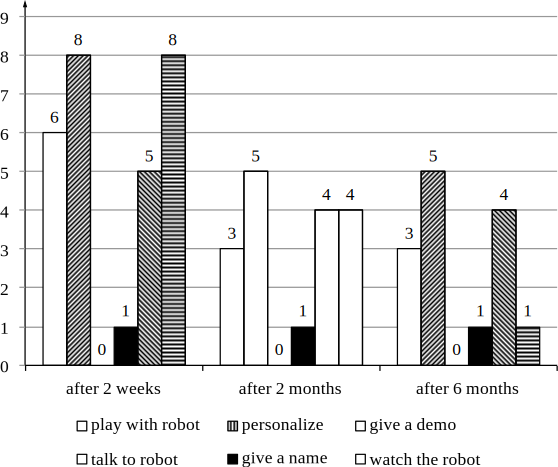
\includegraphics[height=7cm]{roomba-activities}
                \caption{Activities related to Roomba, \textit{n = 9 households}}
                \label{fig:roomba-activities}
        \end{subfigure}%
        \hspace{0.5cm} 
        \begin{subfigure}[t]{0.48\columnwidth}
                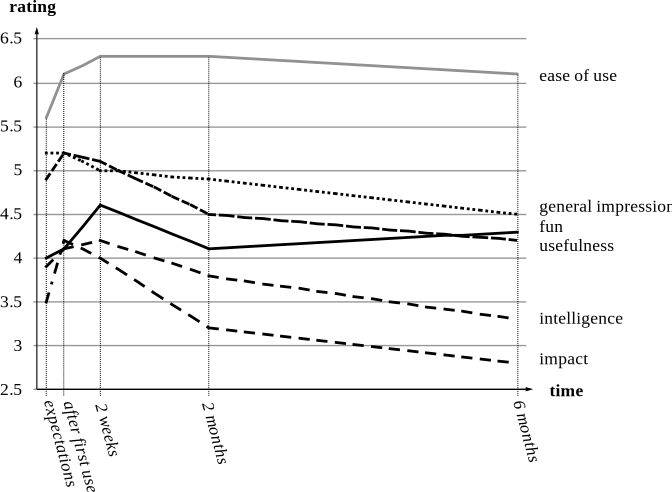
\includegraphics[height=7cm]{roomba-ratings}
                \caption{People's perception of Roomba, \textit{n = 15
                participants}}
                \label{fig:roomba-perception}
        \end{subfigure}
    \caption{Usage and perception of the Roomba vacuum-cleaning robot over a 6
    months period. Qualitative data suggest that people's activities related to
    the robot as well as their perception of the robot change over time.}
    \label{fig:roomba}
\end{figure}

Figures~\ref{fig:roomba-activities} and~\ref{fig:roomba-perception} give a first
perspective on how naive users interact and perceive robots over a long period
of time. Here, \emph{Roomba} vacuum cleaning robots were given to nine
households for a 6-months period. The aim was to explore how people use and
perceive the robot over time, and how they generally live with the Roomba in
their home. At various time points, users were asked to rate their perception of
different features of the robot on a 7-point rating scale. As
Figure~\ref{fig:roomba-perception} shows, some features remained stable over
time (\emph{ease of use} and \emph{fun}), and others decreased: the perceived
\emph{usefulness}, \emph{intelligence} and \emph{impact} on their household.
\emph{intelligence} and \emph{impact} reflect the cognitive engagement of the
user towards the machine: we can assume that one does not care to engage in a
(cognitive) interaction with an artifact perceived as non-intelligent and with
no impact on one's life (and the level of activity pictured in
Figure~\ref{fig:roomba-activities} qualitatively confirms this intuition). Even
if one can argue that the Roomba is not designed to foster interaction, it
raises a first question: how to sustain engagement between a robot and a human
over a long period of time? And, as a pre-requisite to answer, do we actually
understand the psychological phenomenon, and can we effectively account for the
dynamics of these interactions?

Those questions are certainly not new, but paradoxically, while anthropomorphism
is a commonly discussed trait of human-robot interaction, it appears
that we lack formal grounds and models that would account for the long-term
dynamics of these interactions.

\begin{figure}[b]
        \centering
        \begin{subfigure}[b]{0.48\columnwidth}
                \centering
                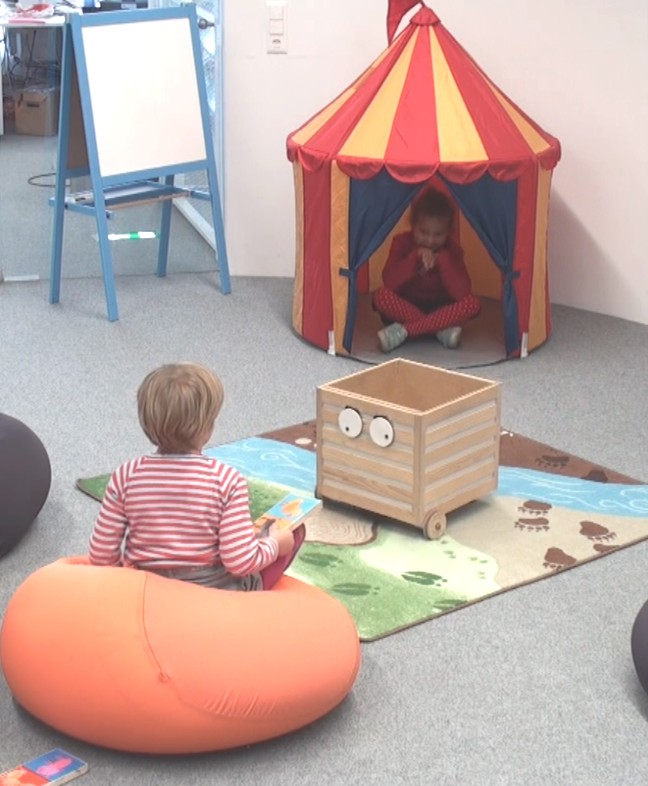
\includegraphics[width=0.75\textwidth]{ranger}
                \caption{Interaction scenario of the \emph{Ranger} domino study:
                the robot toy box Ranger transports domino tiles between the two
                children}
                \label{fig:ranger-expe}
        \end{subfigure}%
        \hspace{0.5cm}
        \begin{subfigure}[b]{0.48\columnwidth}
            
\includegraphics[width=\textwidth]{correlation}
            \caption{\emph{Engagement actions} vs \textit{subjective anthropomorphic
                perception} evidence one cluster of
                high-anthropomorphizers/low-interactors and another group of children who
                interact more with the robot and anthropomorphize it less.}
            \label{fig:qualitative-score}
        \end{subfigure}
        \caption{Children's interaction with Ranger, and their anthropomorphic
        projections onto the robot. Overall, large variations of both children's
        behavior and their perception of the robot were found but seemed to be
        correlated to each other.}
    \label{fig:ranger}
\end{figure}


Figure~\ref{fig:qualitative-score} calls for other initial remarks. This diagram
shows data from a (yet unpublished) study in which 13 pairs of children (4-5
years old) played for about 20 minutes a Domino game with a robot toy box (the
robot was tasked to carry domino pieces from one child to the other,
Figure~\ref{fig:ranger-expe}).  The $x$-axis represents the number of social
interactions between the children and the robot (like talking to the robot or
showing objects), based on video annotations. On the $y$-axis, we have a
synthetic qualitative measurement of anthropomorphic projections onto the robot,
based on two interviews with the children. The correlation between both these
values is significantly \emph{negative}: the more the children engaged into
interaction, the less prone to anthropomorphic projections they were. This
diagram also highlights an interesting cluster of children who did not interact
much with the robot, and still reported a strong anthropomorphic perception of
the robot.

These results may seem counter-intuitive at first sight, and illustrate that the
mechanisms that relate anthropomorphism to adoption and engagement are
non-trivial. In section~\ref{sec:cognition-neuroscience}, we sketch a model of
the cognitive correlates of anthropomorphism that partially account for these
results.


\subsection{Towards a formal understanding of anthropomorphism}

These first remarks lead to the main question we attempt to address in this
article: how can we understand \emph{anthropomorphism} as a whole, and in such a
way that it supports or improves human-robot interaction?

We propose to discuss anthropomorphism from three complementary perspectives: 

First, by reviewing what anthropomorphism actually \emph{means}: besides an
\emph{artifact-centered} understanding that explains anthropomorphism from the
human-like design of the non-human artifact, it seems important to explicit the
social component, namely a \emph{human-centered} understanding, of
anthropomorphism.

Second, we propose a model, called the \textit{Dynamics of Anthropomorphism} to
understand how anthropomorphism evolves over time
~\citep{lemaignan2014dynamics}.  These dynamics are non-monotonic, and effects
like the \emph{novelty effect} play here a key role.

Finally, we adopt a third perspective on anthropomorphism by investigating its
\emph{cognitive correlates}. Several studies previously showed that we build
instinctive bonds with robots as soon as we attribute animacy, and we also know
from social psychology some of the mechanisms that lead to
\emph{familiarization}. We attempt here to ``connect the dots'', in order to
build a practical model of the cognitive stages we encounter in human-robot
interaction.


\subsection{Terminology used in this article}

We use the term \textbf{anthropomorphism} to describe the \emph{psychological}
phenomenon, which arises in the \emph{social context} of an interaction between
a human agent and a non-human agent, in our case, a robot (see Figure
\ref{fig:anthropofig}). We use this term to refer to both people's tendency to
\textit{perceive} human-like characteristics, and to the tendency to
\textit{ascribe} or \textit{attribute} such human-like characteristics to the
agent or artifact. Besides, we call {\bf anthropomorphic effects} the
\emph{observable manifestations} of anthropomorphism, \ie the human's behaviors
and actions toward a non-human agent that reflect the underlying cognitive
process of anthropomorphizing.

However, despite the fact that ``anthropomorphism'' literally means ``human
form'' we propose that the term should \textit{not} be used to refer to the
\textit{form / design} of a non-human agent or artifact. To refer to an
imitation of human-like \textit{form / design} of artificial agents, we propose
to use the term \textbf{anthropomorphic design}. This explicit terminology
prevents the commonly encountered confusion between anthropomorphism as a
psychological, subjective phenomenon, and the external, objective factors that
\emph{influence} the phenomenon itself.

In the following, we might use the terms \emph{form} and \emph{design}
interchangeably. Note that the terms \textit{form} or {\it design} do not only
refer to the shape (how it looks like) but to the total expression of the
artifact~\citep{bartneck_shaping_2004}. \citet{disalvo_hug:_2003} argues that
\textit{form} includes the physical shape, materials, and behavioral qualities
of the product. The behavioral aspect is of special importance for interactive
systems that show some degree of autonomy (independence).  Several categories of
anthropomorphic form exist, with no common agreement on the borders and
transitions between those: anthropomorphic, zoomorphic, caricatured, functional
\citep{fong_survey_2003}.


\subsection{Article overview}

The remainder of this article is organized as follows.  According to the three
perspectives that we take, we first (in Section \ref{sec:anthropomorphism}) aim
to establish a common ground in the understanding of anthropomorphism. We review
literature from several relevant domains and integrate the different
explanations into an understanding of anthropomorphism as a multi-factor
phenomenon.  Based on this, Section~\ref{sec:our-ideas} proposes a new
conceptual model of the \textit{Dynamics of Anthropomorphism}. This model
describes the variances and dynamics of people's tendency to anthropomorphize an
artificial agent, such as a robot.  Then Section
\ref{sec:cognition-neuroscience} presents a cognitive and neuroscience
perspective on anthropomorphism to consolidate our considerations and the
proposed model.  Section \ref{sec:measuring} looks at how these models can be
operationalized, and in particular, what are the tools at hand to measure
anthropomorphism. Finally, Section \ref{sec:conclusion} concludes this article
and offers starting points for further research on anthropomorphism and the
effect of the human-like design approach in robotics.


%%%%%%%%%%%%%%%%%%%%%%%%%%%%%%%%%%%%%%%%%%%%%%%%%%%%%%%%%%%%%%%%%%%%%%%%%
%
%
%
%		WHAT IS ANTHROPOMORPHISM
%
%
%
%%%%%%%%%%%%%%%%%%%%%%%%%%%%%%%%%%%%%%%%%%%%%%%%%%%%%%%%%%%%%%%%%%%%%%%%%

\section{The Dimensions of Anthropomorphism}
\label{sec:anthropomorphism}

Literature on anthropomorphism is quite diverse. There exist different and
partly conflicting definitions of the term anthropomorphism, and it still
appears controversial that humans tend to \textit{``see human
in the non- human''} \citep{epley_seeing_2007}.

As anthropomorphism arises in an interaction between a human and a non-human
agent~\citep{persson_anthropomorphism_2000}, one can also take two main
\textit{perspectives} when trying to explain why humans anthropomorphize~\citep{lee_human_2005}: an artifact-centered perspective and a human-centered
perspective (the grey triangles in Figure \ref{fig:anthropofig}).

In the following we will only briefly present the artifact-centered perspective
to explain anthropomorphism. A review of anthropomorphic design of robots can
also be found in~\cite{fink_anthropomorphism_2012}. Then, we provide a more
detailed review and synthesis of literature that applies a human-centered
perspective to explain anthropomorphism. We aim here at providing an exhaustive
picture of this phenomenon, by summarizing theories from developmental
psychology, cognitive science, neuroscience, and social psychology.

\subsection{Overview of the diverse understandings of anthropomorphism}

Naturally, conflicts in how terms are used lead to a diversity of understandings
of the phenomenon which is described.  One reason for this might be that
anthropomorphism is a phenomenon that is studied in very different domains that
might each integrate their own understanding, use the same term to refer to
different things.  Despite the fact that there is no commonly accepted
definition, the terms \textit{anthropomorphism}, \textit{anthropomorphic} or
\textit{human-like} are often used as if their meanings were clear and agreed
upon \citep{persson_anthropomorphism_2000}. It is even argued that these terms
might be misused \citep{duffy_anthropomorphism_2002,epley_when_2008}.  For
instance, some researchers refer to \textit{``the robot's level of
anthropomorphism''} \citep{bartneck_is_2007,feil-seifer_human-robot_2008},
whereas others disagree to such a statement because they understand that a
system or artifact itself does not \textit{``contain anthropomorphism''} but
only gives rise to the process of anthropomorphizing in a given user and
situation. Consequently, \cite{persson_anthropomorphism_2000} conclude that
anthropomorphism emerges in the \textit{interaction} between the technology and
the user, and has to be understood as such. We come back on this point in the
next section.


Another paradox is that, while human's tendency to anthropomorphize is commonly
observed, the phenomenon is at the same time still rather poorly understood
\citep{epley_seeing_2007}. The phenomenon itself has been found to be very
complex, sometimes subtle and as such hard to study
\citep{duffy_anthropomorphism_2002,epley_when_2008}. Besides, it is not clear
how to operationalize and measure anthropomorphism (we discuss this question
toward the end of this article, in Section \ref{sec:measuring}).

Depending on which definition of anthropomorphism is applied, not everything
colloquially labeled as \emph{anthropomorphism} really is anthropomorphism.  For
example, it is not always clear whether a person (may it be an adult or a child)
who gives an anthropomorphic response, believes that the other agent really
thinks or acts like a human or whether he/she is using anthropomorphism in a
metaphoric sense \citep{leeds_childrens_1992}.  This call for explicitely
stating what we mean when talking about anthropomorphism. 

Several attempts have been made to clarify what the psychological phenomenon
\emph{anthropomorphism} actually is.  From a psychology point of view,
\citet{epley_when_2008} explain what anthropomorphism is \textit{not}. For
instance, in their understanding, anthropomorphism does not include behavioral
descriptions of observable actions but it requires going beyond what is directly
observable. They also suggest that anthropomorphism does not merely entail
\textit{animism}, as animate life is not a \textit{uniquely} human-like
characteristic.\footnote{For the whole list and more details, the reader may
refer to the original work \citep{epley_when_2008}.}

As human-likeness itself is manifold and complex, some researchers argue that
there might not just be one single type of anthropomorphism but different levels
or gradations. For instance, \citet{persson_anthropomorphism_2000} proposes to
understand anthropomorphism as a multi-layered phenomenon, namely
\emph{primitive categorization}, \emph{primitive psychology},
\emph{folk-psychology}, \emph{traits}, \emph{social roles}, and \emph{emotional
anthropomorphism}. Correspondingly, \citet{ruijten_introducing_2014} propose to
understand anthropomorphism as a continuum ranging from low to high human
likeness, and to measure it as such.


\begin{figure}
    \centering
    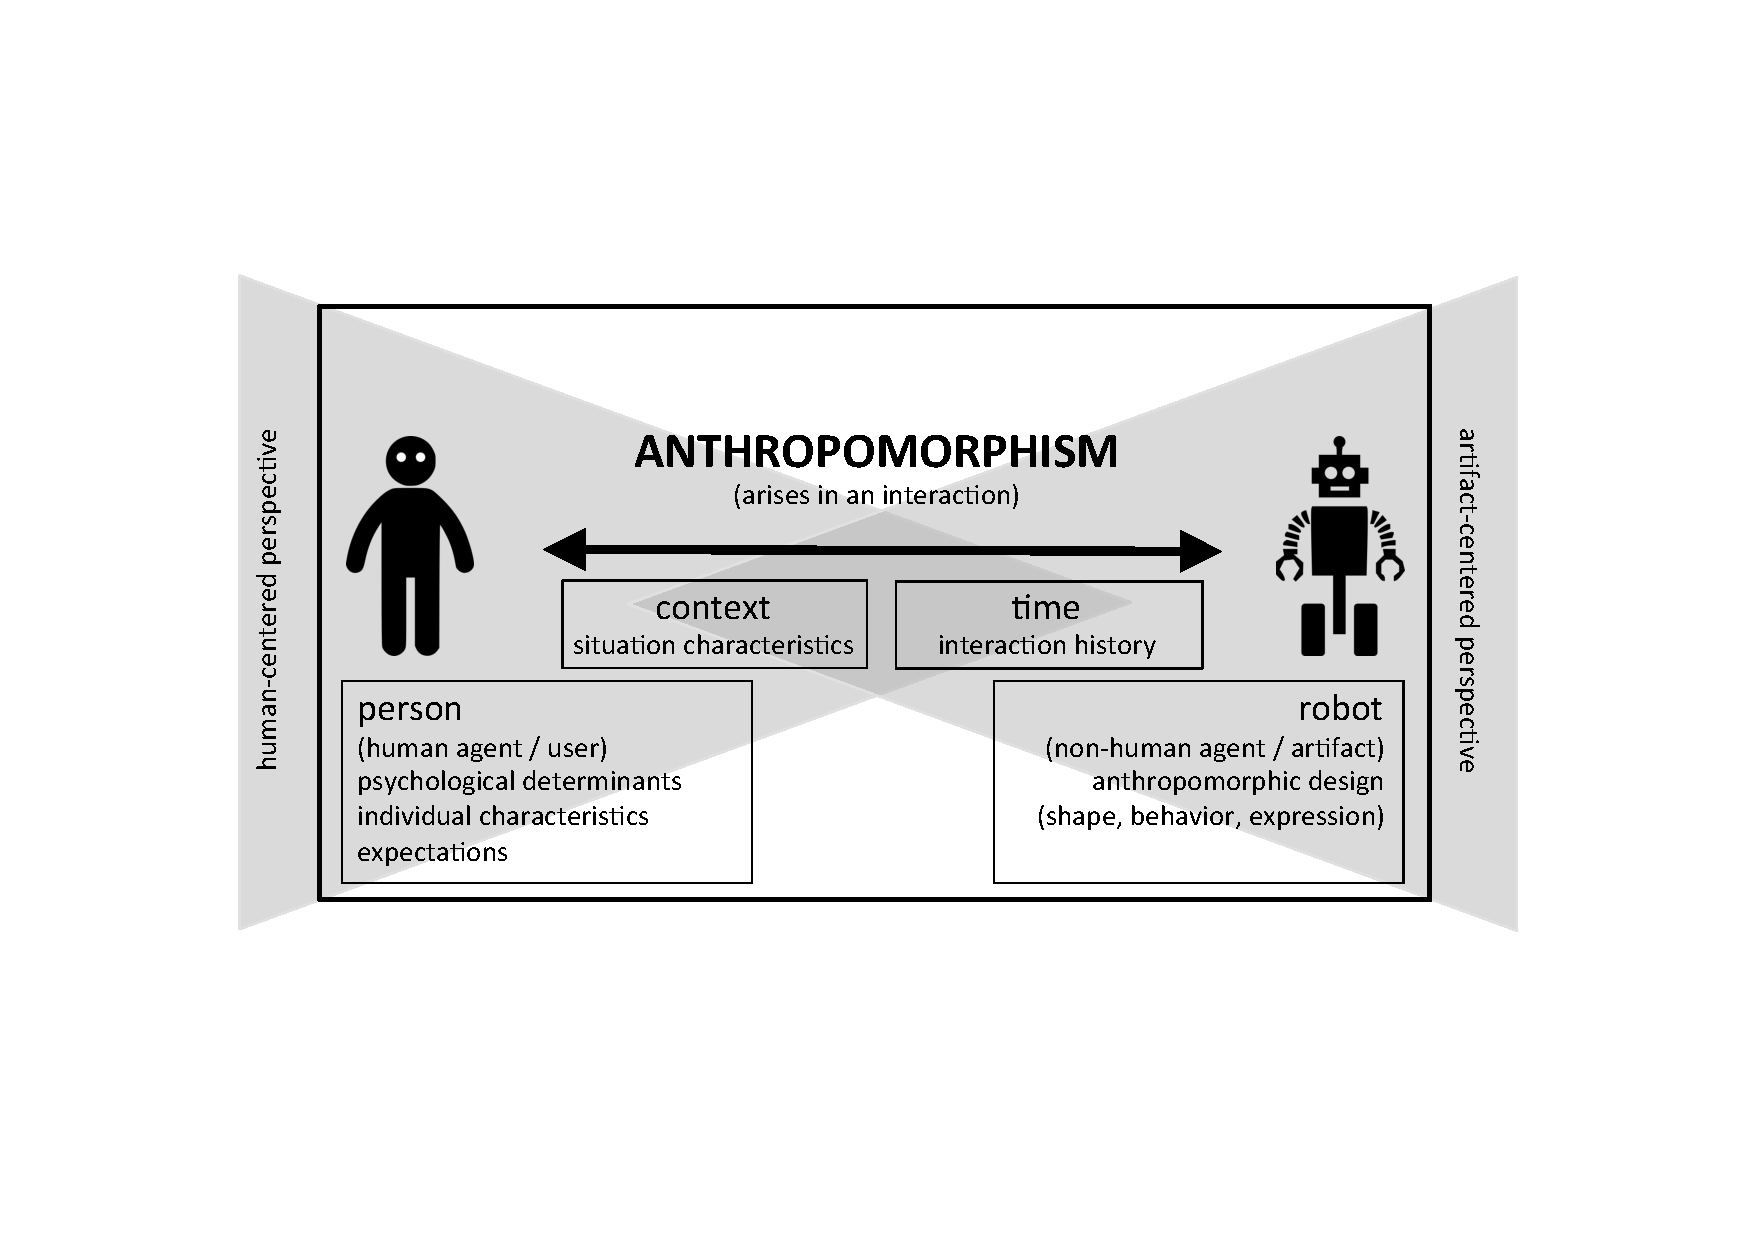
\includegraphics[width=0.75\columnwidth]{anthropo.pdf}
    \caption{Anthropomorphism is a psychological phenomenon which arises in a
        social context, during an interaction between a human agent and a
        non-human agent. One can take two main perspectives when trying to
        explain anthropomorphism: a human-centered and an artifact-centered
        perspective (grey triangles). Several external factors influence the
        anthropomorphism phenomenon. Person- and artifact-related characteristics,
        but also related to the context of use as well as the actual time spent
        interacting with the robot (interaction history).}

    \label{fig:anthropofig}
\end{figure}

%
%\begin{figure}
%    \centering
%    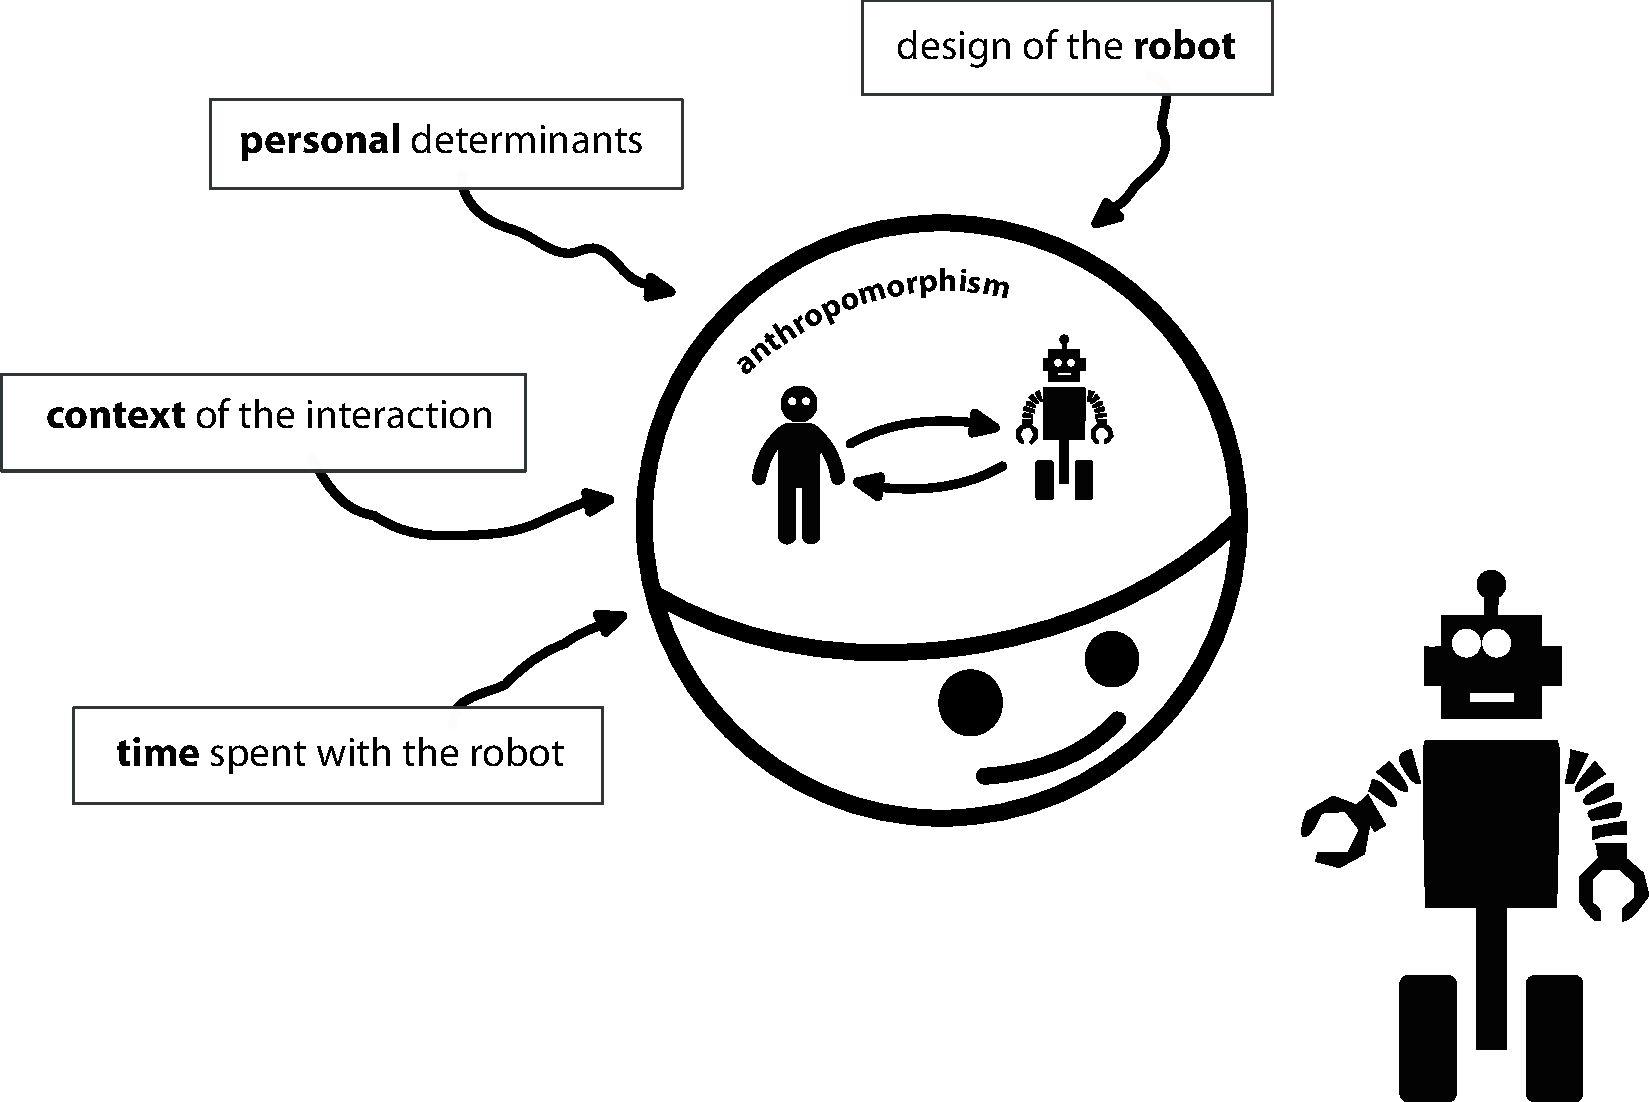
\includegraphics[width=0.75\columnwidth]{in_our_heads.pdf}
%    \caption{[ALTERNATIVE TO FIGURE \ref{fig:anthropofig}] Anthropomorphism is a
%        subjective, psychological phenomenon which arises in a social context, during an
%        interaction between a human agent and a non-human agent. One can take
%        two main perspectives when trying to explain anthropomorphism: a
%        human-centered and an artifact-centered perspective.
%        Several external factors influence the anthropomorphism phenomenon.
%        Person- and artifact-related characteristics, but also related to the
%        context of use as well as the actual time spent interacting with the
%        robot (interaction history).}
%
%
%    \label{fig:anthropofig-alt}
%\end{figure}
%

%%%%%%%%%%%%%%%%%%%%%%%%%%%%%%%%%%%%%%%%%%%%%%%%%%%%%%%%%%%%%%%%%%%%%%%%%
%
%
%
%		WHY DO HUMAN ANTHROPOMORPHIZE
%
%
%
%%%%%%%%%%%%%%%%%%%%%%%%%%%%%%%%%%%%%%%%%%%%%%%%%%%%%%%%%%%%%%%%%%%%%%%%%


\subsection{Artifact-centered perspective on anthropomorphism}

The artifact-centered perspective explains anthropomorphism from the
ascertainable parts of the non-human agent, namely the anthropomorphic form of
it. This section deals with the question how far anthropomorphism can be
explained from the design of the artifact.  One of the most prominent working
hypothesis in this field is the Uncanny Valley hypothesis
\citep{mori_uncanny_1970}. In general, it is proposed that human-like designs of
robots can evoke both positive and negative feelings in a human user. 

The direction of causality in the artifact-centered view goes from the artifact
to the humans: the artifact (or a certain feature of it) \emph{encourages} the
human to anthropomorphize it.  This perspective assumes that humans directly
(mindlessly) respond to life-like and social cues that the non-human agent or
system emits \citep{nass_machines_2000}. Without thoughtful mental processing,
humans tend to simply apply stereotypes and heuristics to the non-human agent,
and in turn apply human-human social schemas and norms to the occurring
interactions.  \cite{takayama_perspectives_2012} proposes to refer to this
immediate (sometimes visceral) sense in a situation as \textit{in-the-moment},
compared to a more distanced cogitation and consideration which she calls
\textit{reflective}. As this distinction implies different cognitive processes,
it is more approriate to apply a human-centered perspective and we will come
back to it later, in section \ref{sec:cognitive-expl}.


%%%%%%%%%%%%%%%%%%%%%%%%%%%%%%%%%%%%%%%%%%%%%%%%%%%%%%%%%%%%%%%%%%%%%%%%%
%
%
%
%		HUMAN-CENTERED PERSPECTIVE: SOCIAL PHENOMENON
%
%
%
%%%%%%%%%%%%%%%%%%%%%%%%%%%%%%%%%%%%%%%%%%%%%%%%%%%%%%%%%%%%%%%%%%%%%%%%%	

\subsection{Human-centered perspective on anthropomorphism}

In contrast to the artifact-centered perspective, in the human-centered
perspective the argumentation is that the human is self-motivated to
anthropomorphize the non-human artifact. As already mentioned, both these views
go hand in hand.

Humans tend to perceive human-like characteristics such as physical appearance,
emotional states, or inner mental states and motivations in non-human agents
that do not have these characteristics themselves, such as animals, natural
forces, religious agents, technological gadgets, or mechanical devices
\citep{epley_when_2008}.\footnote{According to \citet{epley_when_2008}, a
non-human agent can be anything that acts -- or is believed to act -- with
apparent independence.} One common reason for anthropomorphism is that by
perceiving some human-like characteristics in the non-human agent, this agent is
made more \emph{graspable}, \emph{understandable}, \emph{predictable}, and one
can feel \emph{more empathetic} toward it, and possibly one can then anticipate
the agent's behavior. These are central motivations when trying to explain
anthropomorphism, and we will come back to them in more detail later on.
\citet{eddy_attribution_1993} explain that, because of these reasons, people
commonly anthropomorphize their pets, by ascribing mental states, intentions or
feelings to them.\footnote{Interestingly, pet-ownership seems to have a
significant impact on human-robot interaction: several studies suggest that
pet-owners are more likely to anthropomorphize technologies and robots than
non pet-owners} But how can these motivations behind anthropomorphism be
explained from a human-centered point of view?

In the following, we present what we found in reviewing literature that applies
a human-centered perspective on anthropomorphism by building on: \textit{(1)} a
line of research in developmental psychology that studies the attribution of
animacy; \textit{(2)} a line of research in more cognitive sciences that studies
the cognitive processes that underlie anthropomorphism, and \textit{(3)} a
theory that explains anthropomorphism based on psychological factors. 


\subsubsection{Developmental psychology research on the attribution of animacy and intention\\}
\label{sec:developmental-expl}

The phenomenon of attributing animacy and intentions to nonliving objects such
as simple shapes has been intensively studied in developmental psychology. As
mentioned earlier, Piaget found that children tend to ascribe life to the
nonliving. They also tend to interpret physical phenomena in terms of intention
on the part of the non-human subject. For instance children are likely to argue
that \textit{``the sun is hot because it wants to make people warm''}
\citep{leeds_childrens_1992}. In this example it is in fact questionable whether
children really anthropomorphize the sun (believing that it has an intention) or
whether they are using anthropomorphism in a metaphoric sense (because their
conceptions of the world and of the living are not yet fully formed). However,
experiments by \cite{heider_experimental_1944} and
\cite{michotte_perception_1963} showed that also adult participants attribute
animacy and intention to simple things and shapes based on motion. In both
experiments, participants viewed animations of simple shapes, such as circles or
triangles. Asked to describe what they observed, most people developed elaborate
stories, attributing motivations, emotions and relationships between the
objects.\footnote{For more details, the reader may refer to the ``attribution
theory''.}

As mentioned earlier, it seems that there is a natural, relatively spontaneous
reaction that accounts for people's tendency to attribute animacy and intention
to moving shapes, even when there is no similarity of the shape to a human. This
tendency to animize / anthropomorphize is already developed (and even more
distinct) in infants and children. Thus besides the anthropomorphic cues emitted
by the design of the artifact, also developmental stages and people's natural
reaction play a role how far we interpret movements (as one of the
most basic ``life-like'' cues) for instance.


\subsubsection{Cognitive science research, Theory of Mind, and neural correlates
of anthropomorphism\\}

\label{sec:cognitive-expl}

Anthropomorphism and similar phenomenons can also be understood as a thoughtful
process of induction whereby \textit{``people reason about an unknown stimulus
based on a better-known representation of a related
stimulus"}~\citep{epley_when_2008}. In the case of anthropomorphism this means a
person's reasoning about a non-human agent based on the representation of the
self or other humans. A central construct of this perspective is the so-called
\textit{mental model} that a person has (and builds) of the agents he/she is
reasoning about and interacting with. The specific mental model we have about an
artifact / agent basically explains (in our individual way to ourselves) how
this artifact / agent works the way it does.  There are two central aspects
here, that derive from the above quote from Epley.

\textit{(1)} One assumption is that the user is not familiar with the other
agent. This is basically true for all other agents (and entities) but oneself
because we can only be our self. This view is also consistent with the
\emph{familiarity thesis}~\citep{hegel_understanding_2008} which claims that we
understand the world based upon the mental model of the world that we are most
familiar with (\ie our self). Thus, we can best use our self as source of induction
when reasoning about other agents. However, in case we would like to understand
the behavior of a spider, we would probably not use our mental model of a human
(or our self) simply because we do not have many things in common with a spider.
And this is the second central aspect here.

\textit{(2)} One other assumption is based on the anthropomorphic design of the
other agent: if the agent behaves, thus appears, much like a human being (\eg a
robot that emits a human voice), people's mental model of the agent's behavior
is likely to approach their mental model of humans (though the model may differ
in some important aspects).

This cognitive viewpoint on anthropomorphism is important because people's
estimation of an agent's knowledge model and its capabilities affects the way
they relate to it. This holds implications for the resulting interaction with
the system, the user experience, and the acceptance. Previous research examined
the validity of the mental model concept with various kinds of robots
\citep{schmitz_concepts_2011,kiesler_mental_2002}. Findings suggest that people
tend to hold richer mental models of anthropomorphic robots in contrast to
mechanic ones \citep{kiesler_mental_2002}.\footnote{Later in this article,
we may however come to question how far this result is based on
expectations from the human user side, which are likely to be refined
after continued interaction, and after the user gets acquainted with the
robot's behavior.} A similar finding is described in
\cite{hegel_understanding_2008} and \cite{krach_can_2008}. In a user study using
functional magnetic resonance imagery (fMRI), the authors found that
participants implicitly attributed human-like qualities, such as mental states,
to their non-human interaction partner. Indeed, from an early age humans develop
a tendency to explain one's own and others' actions in terms of beliefs, desires
and goals,  called \textit{theory of mind}. The theory of mind allows the
implicit attribution of intentions and other mental states to others
\citep{premack1978does,leslie_pretense_1987,Frith2003}.  The finding of
\cite{hegel_understanding_2008} and \cite{krach_can_2008} was evident at the
behavioral level as well as on the neuro-physiological level: the more the
human-likeness of the artefactual partner increases, the more brain areas
associated with theory of mind  get activated \citep{krach_can_2008}.
Implication of human brain area involved in the inference of others' mental
states has also been shown in response to viewing
non-anthropomorphic/non-humanoid robotic gadgets whose behavior has been
described as unpredictable -- but not in response to those whose behavior was
described as predictable -- a finding also found at the behavioral level
\citep{Waytz2010}.  Interestingly, the grey matter volume of a brain area
related to theory of mind has been correlated to individual's score of
anthropomorphism \citep{cullen2013individual}.

At lower, more automatic, level, robots have been shown to elicit resonance
behaviors in the human brain. Resonance behaviors \citep{Rizzolatti1999} are
mechanisms by which the brain areas involved in the internal representations of
an action, an emotion or a sensation are equally recruited during the perception
of another individual performing the same action or experiencing the same
emotion or sensation.  The neurons showing resonant properties have been called
mirror neurons and have been found in a wide range of modalities (motor,
emotional \etc). Seeing a robotic arm reaching for an object
activates the motor mirror neurons the same way as for seeing a human arm
reaching for the same object \citep{Gazzola2007, oberman_eeg_2007}. However, a
study of emotion perception on a robotic face found reduced activity in
emotional brain area known to have mirror properties in response to the robotic
face compared to a human face \citep{Chaminade2010}. Nevertheless, these authors
showed that when the participants were explicitly instructed to pay attention to
the robot's emotional expression, motor mirror neurons get activated.
Interestingly, using electroencephalography,  it has also been shown that
emotional behavior elicited by a robot face influences the speed of human
responses as well as early brain processes the same way as emotional expression
of a human face did \citep{Dubal2010}.


%


In sum, this branch of research suggests that anthropomorphism implies that
people thoughtfully develop a mental model of agents in their environment and
that they make inferences about these agents based on what is familiar to them
-- themselves, humans and human behavior. This understanding builds on the
theory of mind,  a
person's ability to attribute mental states to oneself and others. 
We briefly reviewed  neuro-physiological evidence of a link between the tendency
to thoughtfully anthropomorphize and the engagement of brain processes involved
in the attribution of mental states to other humans. The human-likeness quality
of the artefactual agent seems to play a role in the involvement of theory of
mind but also the unpredictable feature of the agent behavior alone seems to be
sufficient. Low-level mechanisms of the brain that allow humans to map others'
motor behaviors into their own repertoire are equally elicited when perceiving a
robot's action. It is not yet clear whether humans are processing emotional
signals from a robot the same way as they do for human beings. 


\subsubsection{Social psychology research: a 3-factor theory of anthropomorphism\\}
\label{sec:psychological-factors}

Social psychology, finally, offers theories that apply well to understand
people's motivation to anthropomorphize. Irrespective of the artifact's
characteristics, several psychological determinants have been found to explain a
person's tendency to anthropomorphize. \cite{epley_seeing_2007} present a
\emph{3-factor theory} of when people are likely to anthropomorphize based on
psychological determinants. Namely, the theory suggests that some people are
more likely to anthropomorphize when: 

\begin{enumerate}

    \item ~anthropocentric knowledge is accessible and applicable to the
        artifact (\textit{elicited agent knowledge}),

    \item ~they are motivated to explain and understand the behavior of other
        agents (\textit{effectance motivation}), and

    \item ~they have the desire for social contact and affiliation
        (\textit{social motivation}).

\end{enumerate}

The first factor (\textit{elicited agent knowledge}) is a \emph{cognitive
determinant} of anthropomorphism and based on the idea that a person builds a
mental model (theory of mind) of the other agent. \citet{epley_seeing_2007}
suggest that the process of making inferences about non-human agents is based on
the activation of knowledge about humans (or the self). As mentioned before,
when a person builds a mental model of the other (unfamiliar) agent, the
question here is why does she draw on knowledge about other humans / herself and
not on something else? One basic reasons for this is a person's physical
constraints of being a human and nothing else. Consequently, one has no other
experience than the self and in turn people tend to make inferences about
others' mental states by relying inordinately on their own mental state.
\footnote{Using one's own mental states and characteristics as a guide when
reasoning about other humans is called ego-centrism. In contrast, when using
self-knowledge (or knowledge about humans in general) when reasoning about
non-human agents, this is called anthropomorphism. See
\cite{epley_seeing_2007}.} Also empirical findings suggest that knowledge about
humans in general, or self-knowledge in particular, is likely to serve as a
readily accessible base for induction when reasoning about non-human agents.
This tendency is usually stronger in young children and decreases with cognitive
development and the learning to distinguish the self from other humans, and
non-human agents. 

Both the second factor \textit{effectance} and the third factor
\textit{sociality} are \emph{motivational determinants} of anthropomorphism.
\textit{Effectance} is understood a person's motivation to interact effectively
in one's environment. That means, a person is motivated to be able to
understand, predict, and reduce uncertainty about her environment and the agents
that inhabit it. According to \cite{epley_seeing_2007}, \textit{effectance
motivation} can lead to anthropomorphism, since anthropomorphism serves as one
way to reduce uncertainty and to increase comprehension of events in one's
environment. Again, also according this factor it can be argued that children
are more likely to anthropomorphize than adults. As children are in their early
stages of life, they are likely to feel more uncertain within their environment,
and consequently tend to anthropomorphize more.

The third factor \textit{sociality} describes a person's motivation for social
contact, social connection, and social approval from other agents. In lack of
social connections to other humans (\etc friends, family, colleagues), a person
is more likely to compensate these social connections by anthropomorphizing
non-human agents. In other words \textit{``[...] those who are chronically
lonely should be more likely to anthropomorphize nonhuman agents than those who
are more chronically connected"} \citep{epley_seeing_2007}. Importantly for
anthropomorphism, this social connection often appears to be satisfied by
connections with \textit{``two of the most commonly anthropomorphized non-human
agents, namely pets and religious agents"} \citep{epley_seeing_2007}. Thus, the
motivation of being socially connected increases the tendency to
anthropomorphize non-human agents because first sociality motivation increases
the tendency to perceive human-like characteristics and traits even in non-human
agents, and second it increases the tendency to search for sources of social
connection in one's environment.

%%%%%%%%%%%%%%%%%%%%%%%%%%%%%%%%%%%%%%%%%%%%%%%%%%%%%%%%%%%%%%%%%%%%%%%%%
%
%
%
%		ANTHROPOMORPHISM AS A MULTI-FACTOR PHENOMENON
%
%
%
%%%%%%%%%%%%%%%%%%%%%%%%%%%%%%%%%%%%%%%%%%%%%%%%%%%%%%%%%%%%%%%%%%%%%%%%%	 



\subsection{Summary: Anthropomorphism as a multi-factor phenomenon}
\label{sec:multi-factors}

Summing it up, anthropomorphism is a commonly discussed and studied trait of
human-robot interaction; however its current understanding seems to be stuck.
More concretely, when seeking to understand why anthropomorphism in an
interaction between a human and a non-human artifact happens, most attention is
given to the artifact and/or to the human. We agree that these two are the
essential ``players'' of anthropomorphism (see Figure \ref{fig:anthropofig}).
Indeed and, as outlined before, research has shown that both the human and the
artifact are not only the two players of anthropomorphism but also the two main
``factors'' that can promote or hinder anthropomorphism.

However, we think that this is not the full story. When agreeing to understand
anthropomorphism as a specific type of \textit{experience} that arises in an
\textit{interaction} between a set of user expectations and the external reality
\citep{persson_anthropomorphism_2000}, 
%(see Figure~\ref{fig:anthropomorphism_and_interaction})
it becomes clear that this interaction happens in a specific context, with a
specific history. We think that the context and the history of the interaction
(in Figure \ref{fig:factors} denoted as \textit{time}), are two more factors
that determine anthropomorphism.

\begin{figure}
    \centering
    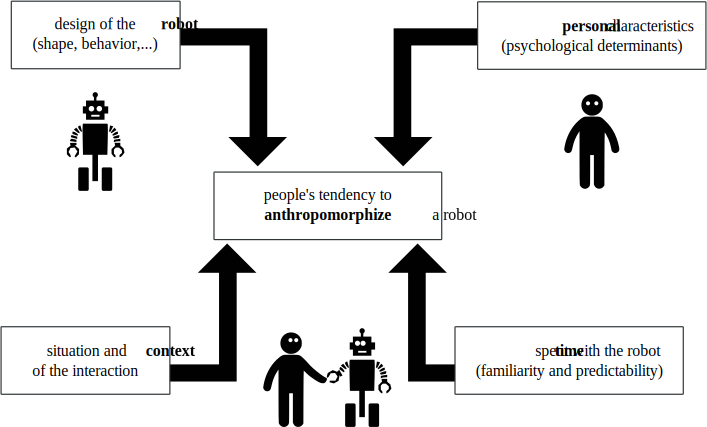
\includegraphics[width=0.7\columnwidth]{factors}
    \caption{Anthropomorphism is a multi-factor phenomenon. How far people tend
    to anthropomorphize a robot is determined by four main factors: the design
    of the robot $(R)$, the personal characteristics of the human user $(H)$, the
    situation and context in which the interaction occurs $(C)$, and the amount of
    time (repeated interaction) that the user spends to familiarize herself with the
    robot $(t)$.}

    \label{fig:factors}
\end{figure}

Consequently, we propose a holistic understanding of anthropomorphism as a
phenomenon which is determined by multiple factors (see also Figure
\ref{fig:factors}):

\begin{enumerate}

\item ~the characteristics of the \textbf{robot's design} (degree of
    anthropomorphic form),

\item ~the psychological determinants in the \textbf{human
    user}~\citep{epley_seeing_2007},

\item ~the characteristics of the \textbf{context / situation} in which the
    interaction occurs, and

\item ~the fact of the user getting familiar with the robot \textbf{over time}
    (duration / history of interaction)

\end{enumerate}

As such, we use in the remaining of the article the notation \Ant[R,H,C,t] to
represent anthropomorphism as a function of the robot's traits $R$, the human
determinants $H$, the characteristics of the interaction context $C$ and the
history of the interaction itself, $t$. This last factor, time, is the focus of
the next section.

%%%%%%%%%%%%%%%%%%%%%%%%%%%%%%%%%%%%%%%%%%%%%%%%%%%%%%%%%%%%%%%%%%%%%%%%%
%
%
%
%				PART 2: OUR IDEAS -- A DYNAMIC PHENOMENON
%
%
%
%%%%%%%%%%%%%%%%%%%%%%%%%%%%%%%%%%%%%%%%%%%%%%%%%%%%%%%%%%%%%%%%%%%%%%%%%

\section{Anthropomorphism: a dynamic phenomenon}
\label{sec:our-ideas}

So far, the HRI community has not much investigated how anthropomorphism in
human-robot interactions evolves over time (during the process of
\emph{adopting} a robot, for instance). Though conflicts were found in the
understanding of what anthropomorphism is, the HRI community more or less
accepted viewing anthropomorphism as a static feature that once observed during
a short-term interaction reflects a sustaining social effect. However, if we
agree that anthropomorphism arises in an interaction, and thus reflects a
specific relation, we cannot accept it as a static phenomenon.

Similarly, \citet{kanda_interactive_2004} point out that relationships among
people evolve over time and, in a similar manner, one can expect people's
attitude toward technological artifacts and their relationship with them to
evolve as well.  In their study, \citet{kanda_interactive_2004} were among the
first to describe empirically \emph{novelty effects} during a long-term study
with an interactive robot in a school.

From a theoretical perspective, we also expect anthropomorphism to change over
time, with growing experience with a robot. As discussed in the previous
sections, anthropomorphism means in essence \emph{reasoning about and perceiving
    something non-human (and unknown or unfamiliar) based on one's
representation of the familiar and well-known concept of being human (or
one-self)}. According to \citet{epley_when_2008}, the basic operations that
underlie these inductive inferences are the \emph{acquisition of knowledge}, the
\emph{activation or elicitation of knowledge}, and the \emph{application of
activated knowledge at the time of the judgment}. By applying knowledge to a
given situation or interaction, one also attempts to correct, adjust, or maybe
integrate less accessible information into a more automatically activated
default representation.  This process of refining the applied knowledge are
natural because a person's knowledge base changes constantly with newly acquired
things. For instance, a person can acquire new knowledge about a robot when
interacting with it. With continued interaction with the unknown system also the
user's expertise with the system grows, and it can be expected that in turn, the
user will become able to better predict the previously unknown system.
Consequently, as the robot becomes more predictable, there is less uncertainty,
and the ``need to anthropomorphize'' the robot decreases (from the
human-centered point of view).

In other words, humans have a motivation to interact effectively in their
environment \textit{(effectance)} \citep{epley_when_2008}.  This means that
humans are motivated to be able to understand and predict the environment and
the agents around them. Thus, a person will seek to become familiar with what is
unfamiliar. Anthropomorphism is encouraged when an agent is unfamiliar.
Consequently, in the process of familiarizing oneself with an agent, the
tendency to anthropomorphize this agent should decrease.

We can not be sure about how exactly the process of familiarization to an
unfamiliar agent (based on continued interaction with the robot) looks like. In
turn, we can not make a precise statement about how continued interaction
decreases anthropomorphism but we suspect there is a link between the two.

In the introduction, we reported on a few selected experimental results that
illustrate how the user tendency to anthropomorphize decreased over time.
Combined with the extensive discussion on the nature and factors of
anthropomorphism that we proposed in section~\ref{sec:anthropomorphism}, we
introduce in the following section a novel qualitative model of the evolution of
anthropomorphism over time, \ie a model of the \emph{dynamics of
anthropomorphism}.


\subsection{A Model of the Dynamics of Anthropomorphism}
\label{sec:dynamics-model}

The phenomenological model of anthropomorphism we propose
(Figure~\ref{fig:dynamics},~\citep{lemaignan2014dynamics}) represents how the
level of ``anthropomorphic effects''~\Ant[R,H,C,t] (\ie the observable
manifestations of anthropomorphism) evolves over a long-term human-robot
interaction.\footnote{We cannot make a precise statement about how long
``long-term'' interaction has to be to be considered as such. It seems to be
practical to not speak of ``several days'' or ``weeks'' but to rather consider
the duration and frequency of the actual interactions with the artifact. One
could probably call this the ``interaction history''.}

While the model primarily considers \emph{long-term interaction} -- direct
(non-mediated), repeated interaction with the same robot, over an extended
period of time (typically longer than a week), we also formally introduce a
so-called \emph{novelty effect}~\citep{kanda_interactive_2004} that models the
first phase of human-robot interaction, during which a specific increase of
anthropomorphic interactions is observed.

In the \emph{Dynamics of Anthropomorphism} model, anthropomorphism is quantified
by a \emph{normalized level of anthropomorphic effects} $\antNorm[R,H,C,t] =
\frac{\ant[R,H,C,t]}{\antMax}$: because anthropomorphic effects are often
qualitative and difficult to quantify on an absolute scale, we present them as a
normalized value, that spans from a minimum (no anthropomorphic effects:
$\ant=0$) to a maximum (noted \AntMax, with $t_{max} = \operatorname{arg\,max}_t
\, \ant[t]$). For the sake of readability, we will use \Ant in the following
sections to refer to the normalized level of anthropomorphic effects. Note also
that we discuss in Section~\ref{sec:measuring} possible methodologies for the
quantitative and qualitative assessment of anthropomorphic effects.

The actual maximum value of anthropomorphic effects depends on each unique
combination of a human, a robot, a situation and several other factors we
introduce below. Thus, the maximum value varies according to the specific
characteristics of these factors. Figure~\ref{fig:dynamics} pictures this
maximum value at $t_{max}$, which actually corresponds to what we call the
novelty effect peak.\footnote{We assume that there is a peak in the human's
experiences of the novelty effects of the unfamiliar system. Further, we suspect
that this novelty peak comes along with the maximum value of anthropomorphic
effects.} The general \emph{shape} of the curve remains however the same and
depicts the evolution of anthropomorphism over time, \ie the general dynamics of
anthropomorphism.

\begin{figure*}[htb]
\centering


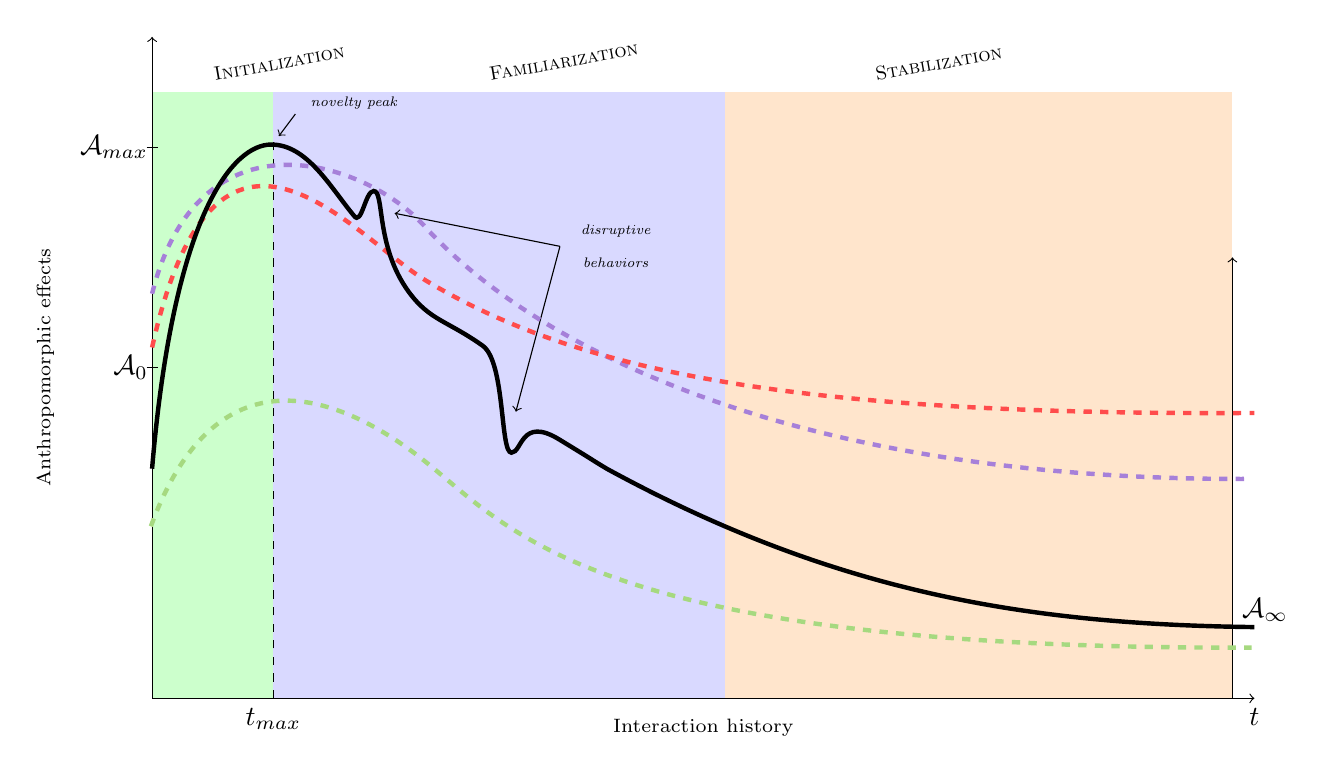
\begin{tikzpicture}[scale=1.4]

% background shading
\path[fill=green!20] (0,0) rectangle (1.1,5.5);
\path[fill=blue!15] (1.1,0) rectangle (5.2,5.5);
\path[fill=orange!20] (5.2,0) rectangle (9.8,5.5);
\draw(0.5,5.5) node[anchor=south west, rotate=10] {\scriptsize \sc Initialization};
\draw(3,5.5) node[anchor=south west, rotate=10] {\scriptsize \sc Familiarization};
\draw(6.5,5.5) node[anchor=south west, rotate=10] {\scriptsize \sc Stabilization};
% horizontal axis
\draw[->] (0,0) -- (10,0) node[anchor=north] {$t$};
\draw(5,-0.1) node[anchor=north] {\scriptsize Interaction history};


% vertical axis
\draw[->] (0,0) -- (0,6) node[anchor=east] {};
\draw(-0.8,3) node[rotate=90,anchor=south] {\scriptsize Anthropomorphic effects};

\draw (-0.05, 3) -- (0.05, 3) node[anchor=east] {\ICA};
\draw (-0.05, 5) -- (0.05, 5) node[anchor=east] {\AntMax};

% vertical axis - end
\draw[->] (9.8,0) -- (9.8,4) node[anchor=east] {};
\draw (9.8, 0.8) node[anchor=west] {\SLA};


\draw[<-] (1.15,5.1) -- (1.30,5.3) node[anchor=east] {};
\draw (1.35,5.4) node[anchor=west] {\tiny \it novelty peak};

\draw[dashed] (1.1, 0) -- (1.1,5.1);
\draw (1.1,0) node[anchor=north] {$t_{max}$};

%\draw[dotted] (0, 5) -- (6.2,5);
%\draw[dotted] (0, 3) -- (6.2,3);
%\draw[<->] (6.1,3) -- (6.1,5) node[sloped, above, midway] {$\Delta_{a}$};

\draw[<-] (2.2,4.4) -- (3.7,4.1) node[anchor=east] {};
\draw[<-] (3.3,2.6) -- (3.7,4.1) node[anchor=east] {};
\draw (3.8,4.1) node[anchor=west, align=center] {\tiny \it disruptive\\ \tiny
\it behaviors};
%%%%%
%% CURVES
%%%%
\begin{scope}[yscale=-1,shift={(-0.125,-0.46)}]
    \draw[ultra thick, green!70!red!50, dashed] svg[scale=1cm] "M 0.114,-1.1 C 0.733,-2.79 1.88,-2.23
    2.51,-1.76 3.34,-1.14 3.94,0.02 10.1,0";

    \draw[ultra thick, blue!70!red!50, dashed] svg[scale=1cm] "M 0.125,-3.21 C 0.549,-4.91 2.05,-4.42
    2.59,-3.83 3.57,-2.74 5.93,-1.51 10.1,-1.53";

    \draw[ultra thick, red!70, dashed] svg[scale=1cm] "M 0.12500001,-2.7222489 C 0.70533638,-5.3401235 1.9431386,-3.7307246 2.608741,-3.3299187 c 1.3619528,0.8201274 3.3166657,1.2251393 7.515191,1.2014756";

    \draw[ultra thick] svg[scale=1cm] "M
    0.125,-1.622832 c 0.19887378,-2.35086 0.74751962,-2.9373641 1.0765913,-2.9404859 0.3290717,-0.00312 0.5370891,0.383599 0.754419,0.6452353 0.069872,0.099803 0.1021612,-0.2231749 0.1792538,-0.2238964 0.099707,0 0.013454,0.4985362 0.3173383,0.9139831 0.1911917,0.2612926 0.3444354,0.2578391 0.6711932,0.4894291 0.2058265,0.1458798 0.1571532,0.9762306 0.2615031,0.9702183 0.097182,0 0.083295,-0.3336208 0.4330446,-0.1199242 0.4306401,0.2631203 0.216699,0.1355642 0.4296663,0.2647074 2.0858202,1.13836043 3.8496455,1.41300027 5.8769904,1.43753027";



\end{scope}

\end{tikzpicture}

\caption{\textbf{Conceptual model of the dynamics of anthropomorphism}. We
    distinguish three main phases: \emph{initialization}, \emph{familiarization}
    and \emph{stabilization}, preceded by a \emph{pre-interaction} phase. The
    pre-interaction phase is characterized through an \emph{initial capital of
    anthropomorphism} (ICA, noted \ICA).  Once the interaction starts, the level
    of anthropomorphism increases due to the \emph{novelty effect}, and then
    decreases to reach a \emph{stabilized level of anthropomorphism} (SLA, noted
    \SLA). \ICA and \SLA may vary depending on the user (and his/her
    expectations), the robot and the context of interaction.  During the
    interaction, unpredicted behaviors of the robot (\emph{disruptive
    behaviors}) may lead to local increases or decreases of the level of
    anthropomorphic effects. The duration of these phases may vary and the
    overall shape of the curve is unique to each human interacting with a
    specific robot in a given context, as depicted by the alternative curves.}

\label{fig:dynamics}
\end{figure*}

\subsection{Three phases}
\label{sec:phases}

We distinguish three main phases that describe the evolution of the
anthropomorphic effects in a long-term human-robot interaction. They are
depicted in different shades in Figure~\ref{fig:dynamics}.

\subsubsection{Initialization Phase\\}

The \textit{Initialization Phase} starts with the so-called \textit{Initial
Capital of Anthropomorphism} ($ICA$), which corresponds to \ICA (value of \Ant
at time point $0$). This value considers the multiple factors presented in
Section~\ref{sec:multiple-factors}, thus it is composed by factors of the human
$H$, the robot $R$, and the context of use $C$. As such, \ICA describes the
value of anthropomorphic effects that can be expected to occur during the first
contact between the human and the robot in a given situation. During this first
phase, pre-conceptions and initial expectations as well as previous experience
of the user with other similar types of robots and similar contexts can have a
strong impact and influence the general tendency to anthropomorphize.

During the \textit{Initialization Phase} we expect an increasing value of $A$
that may be partly due to the so-called \textit{effects of novelty} of the
robot. Such effects have been described with interactive technologies in general
\citep{rogers_diffusion_1995}, and also in several long-term HRI studies in
workplaces \citep{huttenrauch_fetch-and-carry_2003,mutlu_robots_2008}, in
schools and public places
\citep{gockley_designing_2005,kanda_communication_2005,kanda_interactive_2004},
and elder care centers \citep{sabelli_conversational_2011}. Also long-term
studies of domestic robots have shown similar effects and found that after some
time people's interest, engagement, and fascination of the robot decreased
\citep{sung_robots_2009,sung_domestic_2010,fernaeus_how_2010,fink_living_2013}.

What type of anthropomorphic effects are typical during the
\textit{Initialization Phase}? In our own work, we observed that users
spontaneously tend to talk directly to the robot (though the user knows that the
system is not be able to recognize speech), for instance, by greeting the robot,
asking questions to it, giving it nick-names or ascribing a gender, praising the
robot, commenting on its performance in general, and giving commands. Also, the
use of point gestures and waving at the robot were fairly common among
participants of our studies, as well as ascribing gender and some personal
preferences or intention to the robot. (Note that we did not even use an
anthropomorphic robot but a Roomba vacuum cleaning robot.)

In general, it appears that anthropomorphism during the \textit{Initialization
Phase} is a commonly observed phenomenon. But we would like to stress again that
most of these effects are likely to fade out over time.

\subsubsection{Familiarization Phase\\}

In the \textit{Familiarization Phase} the user gets acquainted and familiar with
the robot and with using the robot, and hence the tendency to anthropomorpize
decreases. This phase typically starts as the local maximum value of
anthropomorphic effects that are enhanced by the novelty of the robot start to
wear off. The user may think that he/she faces an agent that aims at
``human-level intelligence'' (to take McCarthy's words). This is a transient
state that quickly vanishes as the user recognized that the behavior of the
robot is generally \textit{predictable} and possibly \textit{deceptive}. For
instance, the robot produces verbal utterances (it ``talks'') but it does not
understand when we talk; or the robot is endowed with eyes but does not
recognize the objects we show it.

\paragraph{Disruptive behaviors.}

We call \emph{disruptive behaviors} any behavior exhibited by the robot hat
appears unexpected to the user: for instance, a robot may usually follow always
the same route to go from one place in a house to the other, but suddenly it
might change the route. The actual underlying reason may span from a bug to the
detection of a new obstacle, but as long as this reason is not immediately
intelligible to the user, the behavior counts as \emph{disruptive}. We further
discuss the role of disruptive behaviors in cognitive terms in Section
\ref{sec:disruptive}.


\subsubsection{Stabilization Phase\\}

During the \textit{Stabilization Phase} the value of $A$ tends to stabilize over
a longer time, to reach a value that we call the \textit{Stabilized Level of
Anthropomorphism} ($SLA$), which corresponds to \SLA. The value that the
$SLA$ approaches is unique for each user interacting with a specific robot in a
given situation. \SLA may approach $0$, when no anthropomorphic effects
are observed anymore, for instance, when the user is interacting with the robot
in a routine way and he/she does not project any human-like traits unto the
robot\footnote{The robot may have become \textit{``invisible in use''}
\citep{takayama_toward_2011}.} As such, the $SLA$ stands for the long-term
lasting value of anthropomorphism.  We proposed that \SLA (the value
corresponding to the $ICA$) is built on multiple factors (see
Section~\ref{sec:multiple-factors}) and similar \SLA is based on these
factors, however taking into account the \textit{interaction history} $t$ that
the user has with the robot.  Note that the $ICA$ and the $SLA$ are generally
not correlated. A person may initially have a high potential of
anthropomorphizing (high \ICA), for instance a highly anthropomorphic robot,
but subsequently get disappointed by the actual capabilities of it and stop
explaining it in terms of human-like characteristics (low \SLA). Another
user may however create lasting affective bonds with the same robot and may
continue to anthropomorphize the robot (high \SLA).



%%%%%%%%%%%%%%%%%%%%%%%%%%%%%%%%%%%%%%%%%%%%%%%%%%%%%%%%%%%%%%%%%%%%%%%%%
%
%
%
%		PART 3: EXPLANATIONS -- COGNITIVE CORRELATES, NEUROSCIENCE VIEW
%
%
%
%%%%%%%%%%%%%%%%%%%%%%%%%%%%%%%%%%%%%%%%%%%%%%%%%%%%%%%%%%%%%%%%%%%%%%%%%

\section{Towards a Cognitive Interpretation}
\label{sec:cognition-neuroscience}

The model that we have introduced so far helps to represent and organize the
\emph{observations} of anthropomorphism. It does so at a conceptual level, and
with a special emphasis on the evolution over time.

This abstract model may contribute to a better understanding of the
\emph{phenomenology} of anthropomorphism, but it does not help to \emph{explain}
the phenomenon. This section proposes to look at the dynamics of
anthropomorphism in terms of \emph{cognitive correlates}: how human cognition
can explain the dynamic nature of our interactions with robots, and what are the
main cognitive stages upon which researchers can build to design better, deeper
human-robot interactions.

We also discuss two specific aspects: the cognitive impact of disruptive
behaviors (section~\ref{sec:disruptive}) on mutual modeling, and how our models
relate to the \emph{in-the-moment} versus \emph{reflective} perspectives on
agency in HRI~\citep{takayama_perspectives_2012}.


\subsection{A Model of the Cognitive Stages of Human-Robot Interaction}
\label{sec:cognitive-model}


\begin{figure}[htb]
\centering
%\resizebox{\linewidth}{!}{
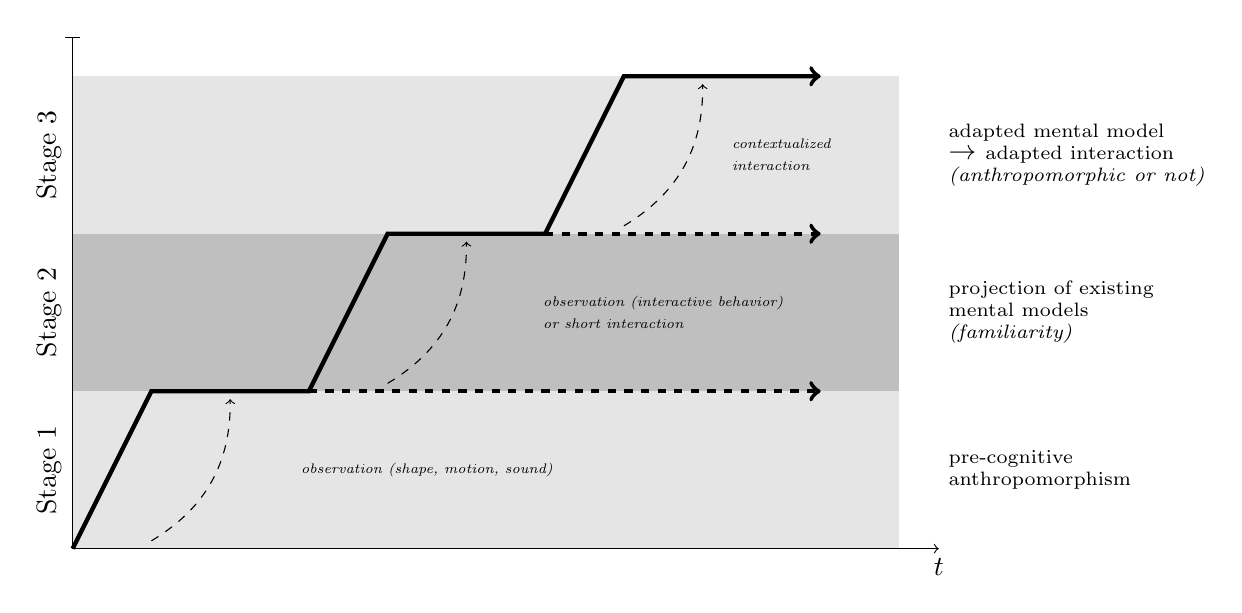
\begin{tikzpicture}
\baselineskip=8pt

\path[fill=gray!20] (0,0) rectangle (10.5,2);
\path[fill=gray!50] (0,2) rectangle (10.5,4);
\path[fill=gray!20] (0,4) rectangle (10.5,6);

\draw (-0.3,1) node[rotate=90] {Stage 1}
      (-0.3,3) node[rotate=90] {Stage 2}
      (-0.3,5) node[rotate=90] {Stage 3};

\draw[->] (0,0) -- (11,0) node[anchor=north] {$t$};
\draw[-|] (0,0) -- (0,6.5) node[anchor=east] {};
% Us
\draw[ultra thick, ->] (0,0) -- (1,2) -- (3,2) -- (4,4) -- (6,4) -- (7,6) --
(9.5,6);
\draw[ultra thick, dashed, ->] (3,2) -- (9.5,2);
\draw[ultra thick, dashed, ->] (6,4) -- (9.5,4);

\draw (11,1) node[align=left, anchor=west]{\scriptsize pre-cognitive\\\scriptsize anthropomorphism}; %label

\draw (11,3) node[align=left, anchor=west] {\scriptsize{projection of existing}\\\scriptsize{mental models}\\\scriptsize{\it (familiarity)}}; %label

\draw (11,5) node[align=left, anchor=west] {\scriptsize{adapted mental
model} \\ $\to$ \scriptsize{adapted interaction}\\\scriptsize{\it (anthropomorphic or not)}}; %label


\draw[dashed,->] (1,0.1) to[bend right] (2,1.9)  node at (4.5,1) {\tiny{\it observation (shape, motion, sound)}}; %label

\draw[dashed,->] (4,2.1) to[bend right] (5,3.9)  node[align=left] at (7.5,3) {\tiny \it observation (interactive behavior) \\ \tiny \it or short interaction}; %label

\draw[dashed,->] (7,4.1) to[bend right] (8,5.9)  node[align=left] at (9,5)
{\tiny \it contextualized\\ \tiny \it interaction}; %label

\end{tikzpicture}
%}
\caption{\textbf{The three cognitive stages of anthropomorphism}: Stage 1 is the instinctive,
sub-cognitive identification of living peers. {\it Empathy} is characteristic
of this stage. After longer observation or short, non-contextualized interaction
(typically, a lab environment), the user reaches Stage 2: the user projects a
mental model he/she is already familiar with onto the robot. After longer {\it
contextualized} interaction (typically, at home), the user enters Stage 3 of
anthropomorphism: the user composes a custom mental model of the robot,
based on experience. This leads to adapted interaction modalities, that may
still be anthropomorphic, or not.}
\label{fig:cognitivemodel}
\end{figure}

We propose three different cognitive stages (Figure~\ref{fig:cognitivemodel}),
which are not mutually exclusive but overlap over time. Note that these three
cognitive stages are related but do not exactly match the \emph{Initialization},
\emph{Familiarization} and \emph{Stabilization} phases introduced in our model
of the dynamics of anthropomorphism.


\subsubsection{Cognitive Processes and Stages\\}

The main underlying cognitive process in anthropomorphism is understood as
perceiving and reasoning about something non-human and unfamiliar based on one's
representation of the familiar and well-known concept of being
human~\citep{epley_when_2008}. This led us to interpret the phases of
anthropomorphic interactions as parallel cognitive phases
(Figure~\ref{fig:cognitivemodel}).

The \emph{Stage 1} is the instinctive, pre-cognitive identification of living
peers. Studies conducted by~\citet{rosenthal-vonderputten_experimental_2013},
who investigated the neural correlates of emotional reactions of humans towards
a robot, supports the idea that humans tend to anthropomorphize robots
intuitively in this pre-cognitive way. {\it Empathy} is characteristic of this
stage~\citep{rosenthalvonderPutten2013neural}.  It is also at this stage that
automatic activation of the human's mirror neurons system  in response to
viewing the robots action and human automatic emotional responses are
contributing at a lower level to the intuitive anthropomorphization.

The intuitive anthropomorphization in the cognitive Stage 1 might be
characteristic of what \cite{takayama_perspectives_2012} calls the
\textit{in-the-moment} perspective on agency with a robot compared to the
\textit{reflective} perspective (see paragraph ``artifact-centered perspective''
in Section \ref{sec:anthropomorphism}).  For instance, we reflectively might
\textit{not} perceive agency in a social robot, but it can feel quite
differently in the moment of interaction. \cite{takayama_perspectives_2012}
argues that neglecting to separate reflective perspectives from in-the-moment
perspectives of agency is one of the major sources of confusion when people talk
and write about anthropomorphism. There seems to be a disconnection between what
people consciously perceive and how they respond to stimuli that they may not
consciously perceive. That means, in the initial phase of interacting with a
novel device \textit{(initialization)} (see Figure \ref{fig:dynamics}) people
might not respond consciously but rather mindlessly \citep{nass_machines_2000},
and in turn anthropomorphize more.  Only after some time of
\textit{familiarization}, they might respond in a more reflective manner (in
turn, the tendency to anthropomorphize might decrease). This can be illustrated
by the fact that people tend to deny interacting with computational systems as
if they were people and yet they respond to computers in many ways that are
remarkably similar to how they respond to people \citep{reeves_media_1996}.
\cite{takayama_perspectives_2012} also applies a cognitive viewpoint on the two
different perspectives of in-the-moment \vs reflective to illustrate
differences. She states that in-the-moment perceptions of agency are largely
shaped by bottom-up perceptual processes, evoking very immediate responses (\eg
to the cues emitted by the artifact's design (``artifact-centered
perspective''). In contrast, according to Takayama, reflective perceptions are
more often shaped by top-down processes because of the nature of reflective
thought.

After a longer observation period (typically including complete action sequences
of the robot) or short interaction (touching, short talk like greetings), we
suggest the human reaches the cognitive \emph{Stage 2}: in this phase, the human
starts building a behavioral and cognitive model of the robot that would support
both the observed and imagined capabilities of the robot.  The \emph{familiarity
thesis}~\cite{hegel_understanding_2008} supports the idea that the human first
projects onto the robot mental models of similar agents he/she is already
familiar with (ranging from animals to human adults, to pets and children). We
hypothesize that the nature of the projected mental model, as well as how deep
the human engages in this projection, might be driven by the same parameters as
we mentioned for the \emph{initial capital of anthropomorphism}
(section~\ref{sec:ica}).  At this stage the human might also change his attitude
towards the robot, paying more attention to social cue than to low-level
behavior which may reinforce the resonance mechanisms. 

The cognitive \emph{Stage 3} is reached after a \emph{contextualized} interaction.
A \emph{contextualized} interaction is \emph{explicitly purposeful} (the purpose
of the interaction, be it purely entertainment, is explicit and conscious to the
human), and takes place in an environment that fosters a stronger cognitive (and
possibly affective/social) commitment from the human in the interaction
(typically, at home). During this interaction, the human iteratively restates
and reshapes his/her behavioral and mental model of the robot (\emph{How does
the robot react to such and such situation/input?  What does the robot know
about me? About itself? About our environment? What can the robot learn?}, etc.).

This mental process depends on the human understanding of the robot's inner
working, as well as his/her own tendency to anthropomorphize (the
\emph{personality} in ICA factor), but at this stage, the \emph{perception} of
the robot (its shape for instance) and its intended \emph{purpose} play a less
important role. It is mostly a human-centric process.  The result of this third
phase would be an iteratively adapted cognitive model of the robot. It is also
at this last stage that the human might have a modified tendency to
anthropomorphize, because he/she has built a full cognitive model of the robot.
Consequently, the human would now be able to attribute appropriate internal
states to the robot through his/her theory of mind.


\paragraph{Relation to the dynamics of anthropomorphism\\}

As mentioned before, the three cognitive stages proposed here do not match with
the three phases in the \emph{Dynamics of Anthropomorphism}.  In particular, the
cognitive Stages 1 and 2 are both included in the \emph{initialization} phase of
the anthropomorphism model. Sub-cognitive anthropomorphism typically
\emph{initiates} the novelty effect by rapidly engaging the human in the
interaction through an initial projected agency, whereas cognitive Stage 2
(projection of familiar mental models) supports the novelty effect by inducing
beliefs that the robot is set up with possibly complex cognitive abilities.

The cognitive Stage 3 also overlaps with the \emph{Familiarization} phase: as
the human gets used to the robot, he/she restates and adapts its
cognitive model of the robot by iteratively reshaping pre-existent, familiar
models until it provides a satisfying support to explain and justify the
observed robot behavior.

A \emph{stable level of anthropomorphism} is reached when the adaptation process
depicted in the cognitive Stage 3 reached a stable state, \ie the user's
experience with the robot is correctly supported by the cognitive model he/she
has built.

Another way to think of the three proposed cognitive stages is to relate them to
the \textbf{user experience} which is characteristic of these three stages. For
instance, \cite{norman_emotional_2003} characterizes  three user experience
dimensions (related to emotional attachment), which occur when people use or see
a product for the first time: \emph{(1)} the \emph{visceral level}, which is the
first impression of a product based on its experience; at this level people do
not think about a product but make spontaneous judgments; \emph{(2)} the
\emph{behavioral level}, in which people use and experience the product,
appraise its functions, and consider aspects such as usefulness and usability;
\emph{(3)} the \emph{reflective level}, in which consciousness takes part in the
process, and past experiences are taken into account.  In a study which was
carried out in a shopping mall, \cite{weiss_i_2009} explored the emotional
attachment during first time reactions of children and adults with the robotic
dog AIBO. The authors also argue that it is important to understand the
long-term development of people's social bonds to robots.


\subsection{Role of disruptive behaviors}
\label{sec:disruptive}

A cognitive interpretation of anthropomorphism also allows to better interpret
the role of unexpected robot behaviors, that are \emph{disruptive} with respect
to the cognitive process of building a mental model of the robot.

Common observation of naive people (children or adults) interacting with robots
shows that unexpected behaviors of the robot can have a notable impact on
interaction. This is supported by the results from~\citet{Waytz2010}, mentioned
in section \ref{sec:cognitive-expl}, that show that people attribute more easily
anthropomorphic features to artifacts when they have unpredictable behaviors.
Also \cite{short_no_2010} found that variations in a robot's behavior (such that
it is unexpected) influence people's attribution of mental states and
intentionality to a robot. Participants who were playing the
``rock-paper-scissors'' game with a robot that tried to cheat (either verbally
or in its action), displayed a greater level of social engagement and made
greater attributions of mental states.  However, an unexpected (disruptive)
robot behavior might also have a negative effect on user's engagement with the
robot. For instance, when the user interprets the robot's behavior as a failure,
he/she might lose trust in the robot. \cite{desai_impact_2013} found that in an
interaction scenario, especially early failures of the robot can cause a
dramatically lower real-time trust, compared to middle or late drops of
reliability of the robot.

During a normal interaction with the robot, the user iteratively refines his/her
own model of the behavior of the robot. As explained in previous sections, as
the user improves his/her model of the robot's actions, he/she also improves the
ability to predict the actions and thus, the user tends to anthropomorphize
less.

We emit the hypothesis that an unexpected robot behavior might lead the user to
suddenly restate his/her behavioral model of the robot and will temporarily lead
to an increase or decrease of the level of anthropomorphism (depicted by the
spikes in Figure~\ref{fig:dynamics}).

\begin{figure}
    \centering
    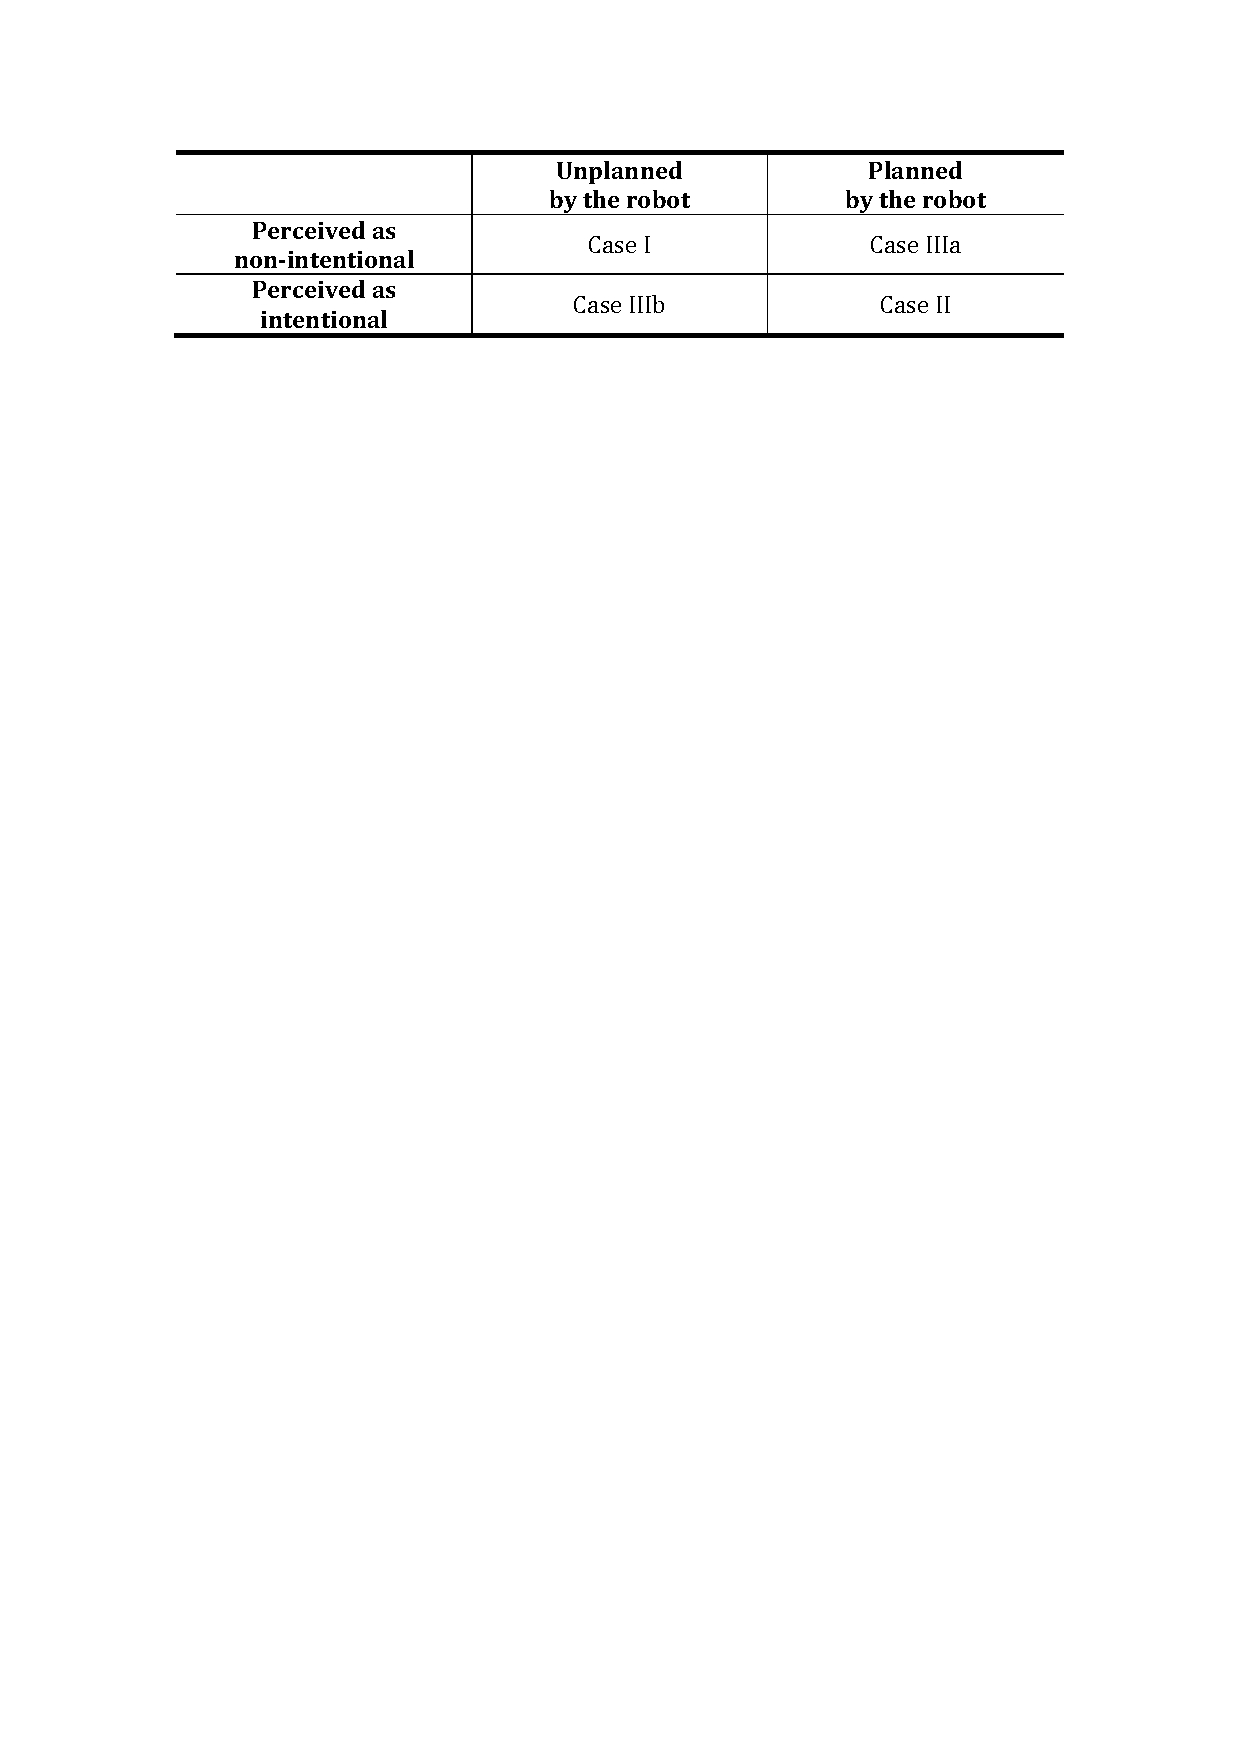
\includegraphics[width=0.75\columnwidth]{un-expected-behavior.pdf}
    \caption{Behaviors of the robot that are unexpected by the user may be intentional
    (the robot has planned the behavior) or not (typically, a failure:
    misdetection, bug,...). Independently of that, the behavior may be
    \emph{perceived} by the user as intentional or not.}

    \label{fig:perceptionUnexpectedBehavior}
\end{figure}


When talking about \emph{unexpected robot behaviors}, several distinct cases
must however be considered, summarized in
Table~\ref{fig:perceptionUnexpectedBehavior}.

If the unexpected behavior is not planned, and perceived as such by the human
(case I), the human can interpret that the robot is able to fail. If the robot
explicitly states its failure (for instance, by saying ``I'm lost!''), the
behavior is then called \emph{transparent} \citep{kim_who_2006}, and the user
may hypothesize that the robot has \emph{introspective} capabilities (it can
reflect on its own internal state), which may lead to higher anthropomorphic
projections.  On the contrary, if the robot shows no sign of recognizing its own
failure, the user may ascribe a lower level of anthropomorphism to the robot.

In case II, the robot voluntary executes a behavior that is unexpected by the
human, and the human perceives it rightfully as an \emph{intentional} behavior.
For instance, the human asks the robot to go somewhere, and the robot refuses,
saying ``I do not want to go there''. In that case, we expect to see an increase
of attribution of anthropomorphism due to the human ascribing intentionality to
the robot.

Case IIIa and IIIb correspond to misinterpretations of the robot behavior. Case
IIIb may actually lead to an increased level of anthropomorphism since the human
will (wrongfully) attribute intentionality to the robot, while case IIIa is
expected to lead to a lower anthropomorphism level.  However, in those two
cases, the next occurrence of an expected behavior, if correctly interpreted
(case I or II), is likely to lead to stronger effects due to a larger delta 
between expectations and actual observed behavior. 

%%%%%%%%%%%%%%%%%%%%%%%%%%%%%%%%%%%%%%%%%%%%%%%%%%%%%%%%%%%%%%%%%%%%%%%%%
%
%
%
%				DISCUSSION + FUTURE WORK
%
%
%
%%%%%%%%%%%%%%%%%%%%%%%%%%%%%%%%%%%%%%%%%%%%%%%%%%%%%%%%%%%%%%%%%%%%%%%%%

\section{Measuring anthropomorphism}
\label{sec:measuring}

Most of the experiments that investigate anthropomorphism in HRI are
conducted in controlled lab-settings during a short-term scenario. For instance,
pictures or videos of different robots are shown to human subjects who
subsequently fill in a questionnaire, to assess how far the different types of
robots were perceived human-like. We think that such experimental
settings have limitations for studying a social phenomenon like
anthropomorphism. The critical question is: can anthropomorphism really be
measured in a post-interaction closed questionnaire or by rating scales?
Findings might possibly lead to interpretations that would not be generalizable
to natural settings or real interaction scenarios (which is always an issue in
social science research).

The Godspeed questionnaire~\citep{bartneck_measurement_2008}, and in particular,
its subpart focused on anthropomorphism, is the main validated questionnaire to
assess anthropomorphism. On 5 point semantic differential scales, people are
asked to rate the following constructs: fake \vs natural, machinelike \vs
humanlike, unconscious \vs conscious, artificial \vs lifelike, moving rigidly
\vs moving elegantly. Because the concept of ``human-likeness'' itself is
complex and abstract, \cite{kahn_jr._robotic_2006} suggest to ask for more
concrete constructs that are typical or unique of the concept of
``human-likeness''.  For instance, \cite{ruijten_introducing_2014} propose a
25-item questions to measure various concrete aspects of human-likeness.
Consequently, anthropomorphism can be modeled along a scale that accounts for
lower and higher levels of it.

Still, measuring anthropomorphism (or social engagement with a robot) through
subjective self-reporting remains challenging because the phenomenon is
partially unconscious, its mediation is largely subject-dependent, and we found
the phenomenon generally difficult to verbalize for users.

As a consequence, to reduce subjectivity and still accurately account for
psychological effects, it is necessary to interleave quantitative and
qualitative assessments of anthropomorphic effects.

We present in this section the methodology and techniques that we used to assess
anthropomorphic projections in the child-robot interaction study, called the
Domino study (see Section \ref{sec:field-results}, and Figure \ref{fig:ranger}).

\paragraph{Qualitative and quantitative assessment of anthropomorphism in
human's behavior\\}

Anthropomorphism can possibly be observed in how humans behave toward a
non-human agent (social human-like engagement). Based on video recordings of the
Domino experiment, we acquired both quantitative and qualitative behavioral data
that reflects anthropomorphism.

Quantitative data are acquired by systematic annotations of specific types of
actions in the video records of the interaction. Six classes of interactions
were identified as reflecting active commitment and/or an anthropomorphic
interaction of the user: gestures toward the robot, touching the robot, direct
talk to the robot, showing something to the robot, mistreating the robot (\eg
kicking it), and looking at the experimenter because worried by the robot's
behavior.

By considering the number of occurrences, the duration, and consequently the
frequency of these types of interaction, we can make statements of how far the
robot is anthropomorphized in an interaction (based on quantitative data).

We assessed anthropomorphic interactions qualitatively by looking at specific
instances of human-social cues in the human's behavior, such as: facial
expressions, observable emotional reactions (\eg surprised, high pitch voice or
shouting to the robot), eye-contact with the robot, turn-taking gestures,
greeting (waving) gestures. These are just suggestions of actions that might
reflect anthropomorphism. These actions partly overlap with the quantitative
assessment, however it is generally advisable to combine the two.


\paragraph{Qualitative assessment of anthropomorphism when verbally referring to
the robot (reflection)\\}

The main tools for qualitative measurement of anthropomorphic effect are
questionnaires and semi-structured interviews. We have explored both
rating-scales in a questionnaire, and open questions in an interview.  In the
Domino study, interviews were transcribed and participant's answers to the key
questions that were assessing an anthropomorphic projection onto the robot, were
analyzed. For instance, one question to see how far children would ascribe moral
standing to the robot was \emph{``If you had this robot at home, and you were to
leave for 2 weeks of holidays, would it be ok to leave the robot alone at
home?''}. A point for anthropomorphism was counted, when the participant's
answer indicated an anthropomorphic view of the robot. This process led to a
``qualitative score'' that reflects how far the robot is anthropomorphized.
Table~\ref{tab:domino-questions} summarizes the constructs that we used to
measure how far the robot is perceived as a human-like agent, along with example
questions.


\begin{table}
\centering
\begin{tabular}{lp{10cm}}
    \toprule
    \textbf{Expectations}  &
    \emph{How do you imagine a robot?} \newline
    \emph{What could it look like?} \newline
    \emph{Have you ever seen a robot before?}
    \\
    \midrule
    \textbf{Impression} &

    \emph{When you first saw R, what did you think?} \newline
    \emph{Is R a robot? How do you know?} \newline
    \emph{Did you expect R would come over to you when you call it?} \newline
    \emph{What happened when you put the domino tile in the box?}
    \\

    \midrule
    \textbf{Ascribe intention} &

    \emph{Do you think R could go out the door all by itself?} \newline
    \emph{Does R always obey / come over to you?} \newline
    \emph{Could R do something silly?} \newline
    \emph{Why did R not come over to you when you called it?}
    \\
    \midrule
    \textbf{Ascribe cognitive connections} &


    \emph{Here is a domino tile. Do you think R can see it?} \newline
    \emph{When I say \textit{``Hello R!''}, do you think R can hear it?}
    \\
    \midrule
    \textbf{Ascribe emotional state} &


    \emph{Does R have feelings? Can R be happy or sad sometimes?}
    \\
    \midrule
    \textbf{Social acceptance} &


    \emph{Do you like R? Why (not)?} \newline
    \emph{What do you (not) like about it?} \newline
    \emph{Would you like to have R at home?}
    \\
    \midrule
    \textbf{Companionship} &

    \emph{Could R be your friend? Why (not)?}
    \\
    \midrule
    \textbf{Ascribe moral standing} &


    \emph{Assume you go on a holiday for two weeks. Is it alright to leave R
    alone at home? Why (not)?}
    \\
    \bottomrule

    \end{tabular}

    \textbf{\refstepcounter{table}\label{tab:domino-questions}Table \arabic{table}.} Constructs and questions used during the semi-structured interviews
    with children. The Ranger robot toy box is abbreviated with ``R''. Questions
    related to the construct \emph{expectations} were asked during the
    pre-interview.

     

\end{table}

Some of these questions were taken from previous work done by
\cite{kahn_jr._robotic_2006} an \cite{weiss_i_2009}. In both studies, both
questionnaires and an analysis of behavior were used to assess children's and
adult's engagement with, and perception of the robot. This seems to be a
promising approach to investigate anthropomorphism, as it is also possible to
combine quantitative and qualitative techniques. 

%%%%%%%%%%%%%%%%%%%%%%%%%%%%%%%%%%%%%%%%%%%%%%%%%%%%%%%%%%%%%%%%%%%%%%%%%
%
%
%
%				CONCLUSIONS
%
%
%
%%%%%%%%%%%%%%%%%%%%%%%%%%%%%%%%%%%%%%%%%%%%%%%%%%%%%%%%%%%%%%%%%%%%%%%%%

\section{Conclusion}
\label{sec:conclusion}

Anthropomorphism is a social phenomenon which seems to be natural on one side
and very complex on the other side. It is a mechanism within oneself that makes
a human observer think and treat a non-human agent as if it would have some
human (social) characteristics, and ascribe to it intentions, emotions, or
thoughts, for instance. Understanding the reasons and modalities of
anthropomorphism is thus of prime importance to build a successful and lasting
human-robot interaction.

Based on our previous (and on-going) work, we hypothesized that there are
qualitative differences and dynamics over time in how humans relate to different
types of robots. More concretely, we described that people's perception of
human-likeness in a robot and in turn their human-social engagement with a robot
is based on four main factors: (1) the (anthropomorphic) design of the robot,
(2) individual characteristics of the human user, (3) the context of use /
interaction, and (4) the interaction history (time factor). We further suggested
that people's tendency to anthropomorphize a robot is likely to change over time
with growing experience of the user with the system. 

To formalize the variances in anthropomorphism, we proposed a model that we call
\textit{Dynamics of Anthropomorphism}.  

We introduced the concepts of \emph{initial capital} and \emph{stabilized level
of anthropomorphism} as compound factors to characterize the profile of a given
anthropomorphic (long-term) interaction.

The article also discussed the cognitive correlates of anthropomorphism. We
proposed three cognitive stages corresponding to successive refinements of the
mental models of the robot that the user builds during the interaction. We
showed how these stages relate to observable anthropomorphic effects, and how
they evolve over time.

While subject to discussion and further extensions, we hope that this
contribution consolidates the scientific grounds of anthropomorphism, and
provides support for a better understanding of long-term acceptance of robots in
human environments.


\section*{Acknowledgments}

This research was supported by the Swiss National Science Foundation through the
National Centre of Competence in Research Robotics.

\bibliographystyle{frontiersinSCNS&ENG} % for Science and Engineering articles
\bibliography{dynamics-anthropomorphism}   % name your BibTeX data base


\end{document}
